% Options for packages loaded elsewhere
% Options for packages loaded elsewhere
\PassOptionsToPackage{unicode}{hyperref}
\PassOptionsToPackage{hyphens}{url}
\PassOptionsToPackage{dvipsnames,svgnames,x11names}{xcolor}
%
\documentclass[
  letterpaper,
  DIV=11,
  numbers=noendperiod]{scrartcl}
\usepackage{xcolor}
\usepackage{amsmath,amssymb}
\setcounter{secnumdepth}{-\maxdimen} % remove section numbering
\usepackage{iftex}
\ifPDFTeX
  \usepackage[T1]{fontenc}
  \usepackage[utf8]{inputenc}
  \usepackage{textcomp} % provide euro and other symbols
\else % if luatex or xetex
  \usepackage{unicode-math} % this also loads fontspec
  \defaultfontfeatures{Scale=MatchLowercase}
  \defaultfontfeatures[\rmfamily]{Ligatures=TeX,Scale=1}
\fi
\usepackage{lmodern}
\ifPDFTeX\else
  % xetex/luatex font selection
\fi
% Use upquote if available, for straight quotes in verbatim environments
\IfFileExists{upquote.sty}{\usepackage{upquote}}{}
\IfFileExists{microtype.sty}{% use microtype if available
  \usepackage[]{microtype}
  \UseMicrotypeSet[protrusion]{basicmath} % disable protrusion for tt fonts
}{}
\makeatletter
\@ifundefined{KOMAClassName}{% if non-KOMA class
  \IfFileExists{parskip.sty}{%
    \usepackage{parskip}
  }{% else
    \setlength{\parindent}{0pt}
    \setlength{\parskip}{6pt plus 2pt minus 1pt}}
}{% if KOMA class
  \KOMAoptions{parskip=half}}
\makeatother
% Make \paragraph and \subparagraph free-standing
\makeatletter
\ifx\paragraph\undefined\else
  \let\oldparagraph\paragraph
  \renewcommand{\paragraph}{
    \@ifstar
      \xxxParagraphStar
      \xxxParagraphNoStar
  }
  \newcommand{\xxxParagraphStar}[1]{\oldparagraph*{#1}\mbox{}}
  \newcommand{\xxxParagraphNoStar}[1]{\oldparagraph{#1}\mbox{}}
\fi
\ifx\subparagraph\undefined\else
  \let\oldsubparagraph\subparagraph
  \renewcommand{\subparagraph}{
    \@ifstar
      \xxxSubParagraphStar
      \xxxSubParagraphNoStar
  }
  \newcommand{\xxxSubParagraphStar}[1]{\oldsubparagraph*{#1}\mbox{}}
  \newcommand{\xxxSubParagraphNoStar}[1]{\oldsubparagraph{#1}\mbox{}}
\fi
\makeatother

\usepackage{color}
\usepackage{fancyvrb}
\newcommand{\VerbBar}{|}
\newcommand{\VERB}{\Verb[commandchars=\\\{\}]}
\DefineVerbatimEnvironment{Highlighting}{Verbatim}{commandchars=\\\{\}}
% Add ',fontsize=\small' for more characters per line
\usepackage{framed}
\definecolor{shadecolor}{RGB}{241,243,245}
\newenvironment{Shaded}{\begin{snugshade}}{\end{snugshade}}
\newcommand{\AlertTok}[1]{\textcolor[rgb]{0.68,0.00,0.00}{#1}}
\newcommand{\AnnotationTok}[1]{\textcolor[rgb]{0.37,0.37,0.37}{#1}}
\newcommand{\AttributeTok}[1]{\textcolor[rgb]{0.40,0.45,0.13}{#1}}
\newcommand{\BaseNTok}[1]{\textcolor[rgb]{0.68,0.00,0.00}{#1}}
\newcommand{\BuiltInTok}[1]{\textcolor[rgb]{0.00,0.23,0.31}{#1}}
\newcommand{\CharTok}[1]{\textcolor[rgb]{0.13,0.47,0.30}{#1}}
\newcommand{\CommentTok}[1]{\textcolor[rgb]{0.37,0.37,0.37}{#1}}
\newcommand{\CommentVarTok}[1]{\textcolor[rgb]{0.37,0.37,0.37}{\textit{#1}}}
\newcommand{\ConstantTok}[1]{\textcolor[rgb]{0.56,0.35,0.01}{#1}}
\newcommand{\ControlFlowTok}[1]{\textcolor[rgb]{0.00,0.23,0.31}{\textbf{#1}}}
\newcommand{\DataTypeTok}[1]{\textcolor[rgb]{0.68,0.00,0.00}{#1}}
\newcommand{\DecValTok}[1]{\textcolor[rgb]{0.68,0.00,0.00}{#1}}
\newcommand{\DocumentationTok}[1]{\textcolor[rgb]{0.37,0.37,0.37}{\textit{#1}}}
\newcommand{\ErrorTok}[1]{\textcolor[rgb]{0.68,0.00,0.00}{#1}}
\newcommand{\ExtensionTok}[1]{\textcolor[rgb]{0.00,0.23,0.31}{#1}}
\newcommand{\FloatTok}[1]{\textcolor[rgb]{0.68,0.00,0.00}{#1}}
\newcommand{\FunctionTok}[1]{\textcolor[rgb]{0.28,0.35,0.67}{#1}}
\newcommand{\ImportTok}[1]{\textcolor[rgb]{0.00,0.46,0.62}{#1}}
\newcommand{\InformationTok}[1]{\textcolor[rgb]{0.37,0.37,0.37}{#1}}
\newcommand{\KeywordTok}[1]{\textcolor[rgb]{0.00,0.23,0.31}{\textbf{#1}}}
\newcommand{\NormalTok}[1]{\textcolor[rgb]{0.00,0.23,0.31}{#1}}
\newcommand{\OperatorTok}[1]{\textcolor[rgb]{0.37,0.37,0.37}{#1}}
\newcommand{\OtherTok}[1]{\textcolor[rgb]{0.00,0.23,0.31}{#1}}
\newcommand{\PreprocessorTok}[1]{\textcolor[rgb]{0.68,0.00,0.00}{#1}}
\newcommand{\RegionMarkerTok}[1]{\textcolor[rgb]{0.00,0.23,0.31}{#1}}
\newcommand{\SpecialCharTok}[1]{\textcolor[rgb]{0.37,0.37,0.37}{#1}}
\newcommand{\SpecialStringTok}[1]{\textcolor[rgb]{0.13,0.47,0.30}{#1}}
\newcommand{\StringTok}[1]{\textcolor[rgb]{0.13,0.47,0.30}{#1}}
\newcommand{\VariableTok}[1]{\textcolor[rgb]{0.07,0.07,0.07}{#1}}
\newcommand{\VerbatimStringTok}[1]{\textcolor[rgb]{0.13,0.47,0.30}{#1}}
\newcommand{\WarningTok}[1]{\textcolor[rgb]{0.37,0.37,0.37}{\textit{#1}}}

\usepackage{longtable,booktabs,array}
\usepackage{calc} % for calculating minipage widths
% Correct order of tables after \paragraph or \subparagraph
\usepackage{etoolbox}
\makeatletter
\patchcmd\longtable{\par}{\if@noskipsec\mbox{}\fi\par}{}{}
\makeatother
% Allow footnotes in longtable head/foot
\IfFileExists{footnotehyper.sty}{\usepackage{footnotehyper}}{\usepackage{footnote}}
\makesavenoteenv{longtable}
\usepackage{graphicx}
\makeatletter
\newsavebox\pandoc@box
\newcommand*\pandocbounded[1]{% scales image to fit in text height/width
  \sbox\pandoc@box{#1}%
  \Gscale@div\@tempa{\textheight}{\dimexpr\ht\pandoc@box+\dp\pandoc@box\relax}%
  \Gscale@div\@tempb{\linewidth}{\wd\pandoc@box}%
  \ifdim\@tempb\p@<\@tempa\p@\let\@tempa\@tempb\fi% select the smaller of both
  \ifdim\@tempa\p@<\p@\scalebox{\@tempa}{\usebox\pandoc@box}%
  \else\usebox{\pandoc@box}%
  \fi%
}
% Set default figure placement to htbp
\def\fps@figure{htbp}
\makeatother


% definitions for citeproc citations
\NewDocumentCommand\citeproctext{}{}
\NewDocumentCommand\citeproc{mm}{%
  \begingroup\def\citeproctext{#2}\cite{#1}\endgroup}
\makeatletter
 % allow citations to break across lines
 \let\@cite@ofmt\@firstofone
 % avoid brackets around text for \cite:
 \def\@biblabel#1{}
 \def\@cite#1#2{{#1\if@tempswa , #2\fi}}
\makeatother
\newlength{\cslhangindent}
\setlength{\cslhangindent}{1.5em}
\newlength{\csllabelwidth}
\setlength{\csllabelwidth}{3em}
\newenvironment{CSLReferences}[2] % #1 hanging-indent, #2 entry-spacing
 {\begin{list}{}{%
  \setlength{\itemindent}{0pt}
  \setlength{\leftmargin}{0pt}
  \setlength{\parsep}{0pt}
  % turn on hanging indent if param 1 is 1
  \ifodd #1
   \setlength{\leftmargin}{\cslhangindent}
   \setlength{\itemindent}{-1\cslhangindent}
  \fi
  % set entry spacing
  \setlength{\itemsep}{#2\baselineskip}}}
 {\end{list}}
\usepackage{calc}
\newcommand{\CSLBlock}[1]{\hfill\break\parbox[t]{\linewidth}{\strut\ignorespaces#1\strut}}
\newcommand{\CSLLeftMargin}[1]{\parbox[t]{\csllabelwidth}{\strut#1\strut}}
\newcommand{\CSLRightInline}[1]{\parbox[t]{\linewidth - \csllabelwidth}{\strut#1\strut}}
\newcommand{\CSLIndent}[1]{\hspace{\cslhangindent}#1}



\setlength{\emergencystretch}{3em} % prevent overfull lines

\providecommand{\tightlist}{%
  \setlength{\itemsep}{0pt}\setlength{\parskip}{0pt}}



 


\usepackage{booktabs}
\usepackage{longtable}
\usepackage{array}
\usepackage{multirow}
\usepackage{wrapfig}
\usepackage{float}
\usepackage{colortbl}
\usepackage{pdflscape}
\usepackage{tabu}
\usepackage{threeparttable}
\usepackage{threeparttablex}
\usepackage[normalem]{ulem}
\usepackage{makecell}
\usepackage{xcolor}
\KOMAoption{captions}{tableheading}
\makeatletter
\@ifpackageloaded{caption}{}{\usepackage{caption}}
\AtBeginDocument{%
\ifdefined\contentsname
  \renewcommand*\contentsname{Table of contents}
\else
  \newcommand\contentsname{Table of contents}
\fi
\ifdefined\listfigurename
  \renewcommand*\listfigurename{List of Figures}
\else
  \newcommand\listfigurename{List of Figures}
\fi
\ifdefined\listtablename
  \renewcommand*\listtablename{List of Tables}
\else
  \newcommand\listtablename{List of Tables}
\fi
\ifdefined\figurename
  \renewcommand*\figurename{Figure}
\else
  \newcommand\figurename{Figure}
\fi
\ifdefined\tablename
  \renewcommand*\tablename{Table}
\else
  \newcommand\tablename{Table}
\fi
}
\@ifpackageloaded{float}{}{\usepackage{float}}
\floatstyle{ruled}
\@ifundefined{c@chapter}{\newfloat{codelisting}{h}{lop}}{\newfloat{codelisting}{h}{lop}[chapter]}
\floatname{codelisting}{Listing}
\newcommand*\listoflistings{\listof{codelisting}{List of Listings}}
\makeatother
\makeatletter
\makeatother
\makeatletter
\@ifpackageloaded{caption}{}{\usepackage{caption}}
\@ifpackageloaded{subcaption}{}{\usepackage{subcaption}}
\makeatother
\usepackage{bookmark}
\IfFileExists{xurl.sty}{\usepackage{xurl}}{} % add URL line breaks if available
\urlstyle{same}
\hypersetup{
  pdftitle={Analysis of iPSC Gene Expression (will be changed)},
  pdfauthor={Trinity Minard},
  colorlinks=true,
  linkcolor={blue},
  filecolor={Maroon},
  citecolor={Blue},
  urlcolor={Blue},
  pdfcreator={LaTeX via pandoc}}


\title{Analysis of iPSC Gene Expression (will be changed)}
\usepackage{etoolbox}
\makeatletter
\providecommand{\subtitle}[1]{% add subtitle to \maketitle
  \apptocmd{\@title}{\par {\large #1 \par}}{}{}
}
\makeatother
\subtitle{Final Project}
\author{Trinity Minard}
\date{2025-11-29}
\begin{document}
\maketitle


\section{Introduction}\label{introduction}

The discovery of human induced pluripotent stem cells (iPSCs) by
Takahashi and Yamanaka in 2007 (Takahashi et al., 2007) has
revolutionized the regenerative medicine field. iPSCs are created by
reprogramming somatic cells into an embryonic like state using the
Yamanaka transciption factors: SOX2, OCT4, KLF4, and c-Myc). These cells
have vast capabilities due to their ability to model human development
and diseases \emph{in vitro}, and their potential for patient specific
(autologous) and ``off the shelf'' (allogeneic) cell therapies
(Cerneckis et al., 2024).

With that being said, the characterization of iPSC lines is essential in
any experimental or manufacturing process to ensure consistency in
culturing. This includes analyzing the expression of pluripotency (stem
cell) markers, differentiation markers, and potential chromosomal
abnormalies, to access the population of the culture. This is commonly
done using techniques such as reverse transcriptase or real time
quantitative PCR (RT-qPCR) to analyze mRNA expression (Artyukhov et al.,
2017), or using an antibody based experiment to analyze protein
expression levels, such as Flow Cytometry or immunocytochemistry. When
conducting these experiments, specifically RT-qPCR, reference genes,
also known as housekeeping genes, are used to normalize the expression
of other genes in a sample (Artyukhov et al., 2017). This allows the
expression of genes to be compared across different samples, since it is
presumed that the expression of the housekeeping gene is consistent
across all of the samples. In stem cell samples, however, it has been
found that the commonly used housekeeping genes, such as GAPDH, appear
to fluctuate in iPSC samples (Panina et al., 2020), making it difficult
to achieve accurate normalization data.

RNA Seq is a technique that sequences the entirety of RNA molecules in a
given sample, rather than using gene specific primers or probes as in
RT-qPCR and other techniques. This allows the entire transciptome to be
analyzed, providing a complete picture of the expression of genes in a
sample (Wang et al., 2009). Additionally, gene expression is calculated
by dividing the raw counts of a gene by the total counts in a sample,
eliminating the need for a housekeeping gene. This allows for an
unbiased and quantitiative analysis of millions of genes in sample (Wang
et al., 2009). Despite these advantages, RNA-Seq is far more time
consuming and expensive than RT-qPCR and other experiments, making it
non practical in a manufacturing setting. Therefore, utilizing RNA-Seq
to analyze iPSC samples could provide insight into housekeeping gene
expression, allowing researchers to select ideal reference genes for
their analysis.

A similar study, conducted by Carcamo-Orive \emph{et al.,} investigated
the variability of gene expression across 317 iPSC lines generated from
101 individuals (Carcamo-Orive et al., 2017) and created a publically
avaible data set of their raw RNA Seq data. They found that genetic
variability in the iPSC lines was influenced by a donor specific gene
expression pattern, specifically influenced by donor age, sex, ancestry,
and reprogramming variabilies. iPSCs can also be reprogrammed from a
variety of somatic cells, such as blood, skin fibroblasts, hair
keratinocytes, urine cells, mesencymal stem cells, and bone marrow
(Poetsch et al., 2022). While some somatic cells are easier to obtain
than others, such as blood cells and fibroblasts, iPSCs from these lines
are associated with higher genomic mutations due to the somatic cells'
high turnover rate. Additionally, iPSCs appear to have an epigenetic
memory of their tissue of origin, which has been found to influence
their differentiation (Poetsch et al., 2022). All of these factors, and
many others, could be contributing to the variations in gene expression
in iPSC samples.

This publicly available dataset from Carcamo-Orive \emph{et al.} was
used to analyze the expression of RNA across iPSC samples, with a focus
on the expression of pluripotency markers, differentiation markers, and
housekeeping genes.

\section{Methods}\label{methods}

\subsubsection{Data Cleaning}\label{data-cleaning}

RNA-Seq counts per million data was acquired from Stemformatics using
the Carcamo-Orive (2017) dataset {[}Carcamo-Orive et al. (2017){]}.
Genes in this study were referred to by their Ensembl ID, so gene
information, such as name and RNA type, was integrated from the Emsembl
database.

\emph{further cleaning of the count per million data will be added}

\subsubsection{Figure 1}\label{figure-1}

Genes detected in the RNA Seq counts per million data were grouped into
the following catagories: Protein coding, long non coding RNA (lncRNA),
Small RNAs, Pseudogenes, and Other. A count of the number of genes in
each category was then performed by using the dplyr package (Wickham et
al., 2023) from tidyverse (Wickham, 2023). A fraction and percentage
were then calculated by dividing the count by the sum of count
(i.e.~total count for all categories). The scales (Wickham, Pedersen, et
al., 2025) package from ggplot2 (Wickham, Chang, et al., 2025) was used
to create a pie chart of the counts by RNA category.

\emph{continue methods for following figures \ldots{}}

\section{Results}\label{results}

\begin{figure}

\centering{

\pandocbounded{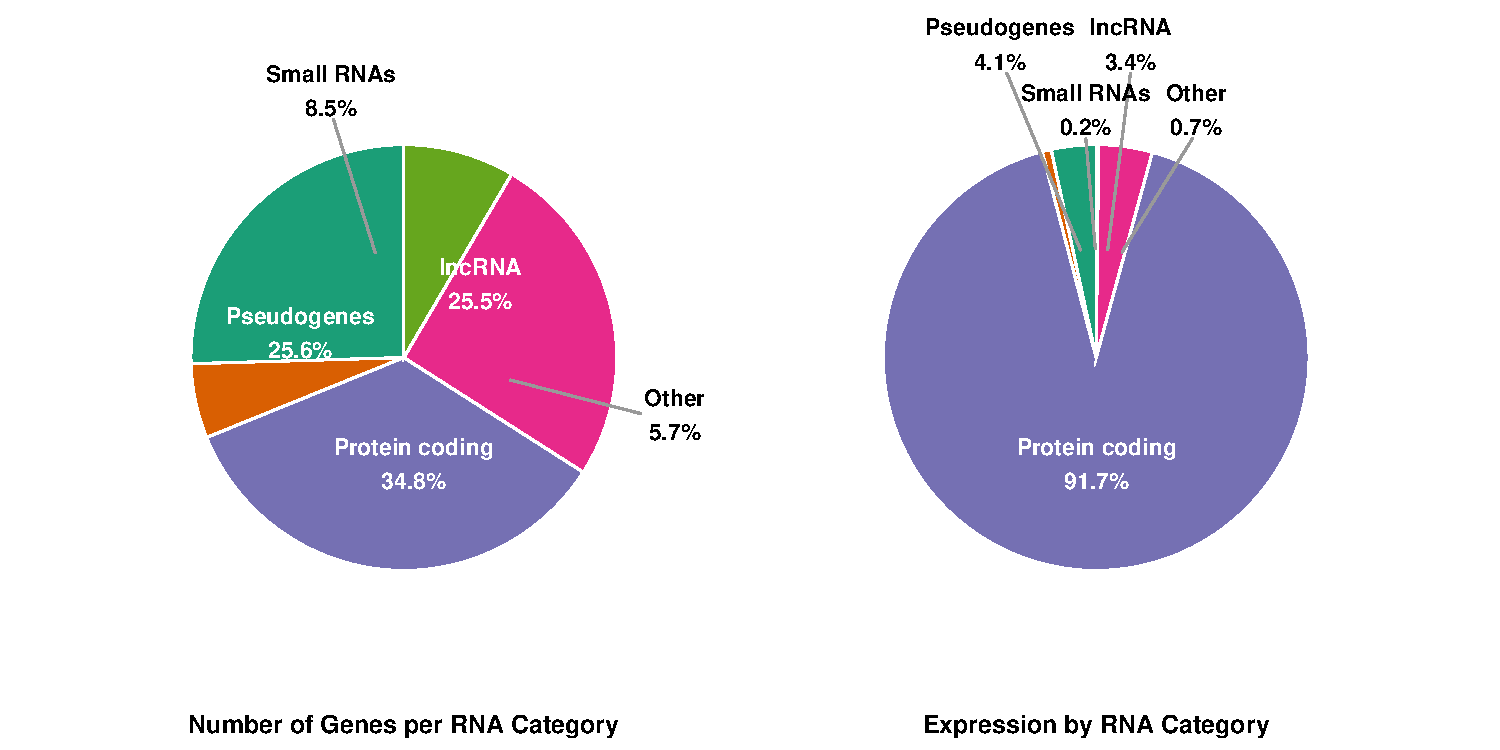
\includegraphics[keepaspectratio]{Final-Project-BIOL806_files/figure-pdf/fig-rna-pie-chart-1.pdf}}

}

\caption{\label{fig-rna-pie-chart}Detected RNA Types in iPSC Sample
Analzyed using RNA Seq. The number of genes detected in each RNA
category from RNA-seq data were counted and plotted as a pie chart
(left). Small categories (\textless{} 2 \%), such as rRNA, tRNA, and
immunoglobulin genes, were combined into an `Other' category. The
expression of genes, using raw count per million data, was averaged by
type of RNA and plotted as a pie chart (right).}

\end{figure}%

\emph{need to fix labels so they line up with slices }

The RNA Seq data is composed of a variety of different types of RNA, as
seen in Figure 1. 34.8\% of read genes are mRNA protein coding genes,
whereas the remaining 65.2\% of the detected genes are not protein
coding and are primary composed of noncoding RNAs and pseudogenes, which
are RNA sequences that look like protein coding genes but are not able
to be translated into a protein. 25.6\% of the detected genes were
pseuodegenes. 25.5\% were long non coding RNA sequences and 8.5\% were
small RNAs, which included snoRNA, snRNA, scaRNA, sRNA, and ribozyme
RNA. 5.7\% were ``Other'' RNAs, which include ribosoal RNA, immunoglobin
genes, T-cell receptor genes, and mitocondrial RNAs. The right pie
chart, on the other hand, displays the expression of these groups. For
each gene for each sample, a count per million number was provided by
Carcamo-Orive \emph{et al.}. This is typically calculated by dividing
the raw count of the gene by the total reads in the sample and
multiplying by one million. The total expression was summed for each
category, and this was graphed in Figure 2, which displays that 91.7\%
of the expression is from protein coding genes. The remaining 8.3\%
accounts for the expression of small RNAs, long non coding RNA,
pseuodgenes, and ``Other'' genes. This is supported by \_\_\_ data from
\_\_\_ article, which saw \_\_\_\_.

Figure X. Will potentially add a PCA plot to identify which variables
strongly influence gene expression.

\begin{verbatim}
Analysis of Variance Table

Response: PC1
           Df  Sum Sq Mean Sq F value Pr(>F)
sex         1    3033  3033.4  0.7567  0.385
Residuals 306 1226658  4008.7               
\end{verbatim}

\begin{verbatim}
Analysis of Variance Table

Response: PC2
           Df Sum Sq Mean Sq F value Pr(>F)
sex         1    713  713.05  0.2855 0.5935
Residuals 306 764263 2497.59               
\end{verbatim}

\begin{verbatim}
Analysis of Variance Table

Response: PC1
            Df  Sum Sq Mean Sq F value Pr(>F)
age_decade   3   21643  7214.5  1.8155 0.1443
Residuals  304 1208048  3973.8               
\end{verbatim}

\begin{verbatim}
Analysis of Variance Table

Response: PC2
            Df Sum Sq Mean Sq F value Pr(>F)
age_decade   3   9096  3032.1  1.2194 0.3027
Residuals  304 755880  2486.4               
\end{verbatim}

\begin{verbatim}
Analysis of Variance Table

Response: PC1
           Df  Sum Sq Mean Sq F value Pr(>F)
age_sex     7   29038  4148.3  1.0365 0.4055
Residuals 300 1200653  4002.2               
\end{verbatim}

\begin{verbatim}
Analysis of Variance Table

Response: PC2
           Df Sum Sq Mean Sq F value    Pr(>F)    
age_sex     7  71066   10152  4.3891 0.0001177 ***
Residuals 300 693911    2313                      
---
Signif. codes:  0 '***' 0.001 '**' 0.01 '*' 0.05 '.' 0.1 ' ' 1
\end{verbatim}

\begin{verbatim}
Analysis of Variance Table

Response: PC1
           Df  Sum Sq Mean Sq F value    Pr(>F)    
race        4  114273 28568.3  7.6996 6.617e-06 ***
Residuals 287 1064872  3710.4                      
---
Signif. codes:  0 '***' 0.001 '**' 0.01 '*' 0.05 '.' 0.1 ' ' 1
\end{verbatim}

\begin{verbatim}
Analysis of Variance Table

Response: PC2
           Df Sum Sq Mean Sq F value    Pr(>F)    
race        4  94361 23590.3  10.251 9.011e-08 ***
Residuals 287 660466  2301.3                      
---
Signif. codes:  0 '***' 0.001 '**' 0.01 '*' 0.05 '.' 0.1 ' ' 1
\end{verbatim}

\begin{verbatim}
\begin{minipage}{0.48\textwidth} \begin{table}[!h]
\centering
\caption{\label{tab:unnamed-chunk-9}Sample counts by Age-Sex}
\centering
\begin{tabular}[t]{lr}
\toprule
Age-Sex Group & Sample Count\\
\midrule
\cellcolor{gray!10}{40s female} & \cellcolor{gray!10}{34}\\
40s male & 8\\
\cellcolor{gray!10}{50s female} & \cellcolor{gray!10}{63}\\
50s male & 41\\
\cellcolor{gray!10}{60s female} & \cellcolor{gray!10}{77}\\
\addlinespace
60s male & 57\\
\cellcolor{gray!10}{70s female} & \cellcolor{gray!10}{17}\\
70s male & 11\\
\bottomrule
\end{tabular}
\end{table} \end{minipage}\hfill \begin{minipage}{0.48\textwidth} \begin{table}[!h]
\centering
\caption{\label{tab:unnamed-chunk-9}Sample counts by Race}
\centering
\begin{tabular}[t]{lr}
\toprule
Race & Sample Count\\
\midrule
\cellcolor{gray!10}{African American} & \cellcolor{gray!10}{20}\\
Asian & 33\\
\cellcolor{gray!10}{Caucasian} & \cellcolor{gray!10}{212}\\
Hispanic & 14\\
\cellcolor{gray!10}{South Asian} & \cellcolor{gray!10}{13}\\
\addlinespace
NA & 16\\
\bottomrule
\end{tabular}
\end{table} \end{minipage}
\end{verbatim}

\begin{figure}

\centering{

\pandocbounded{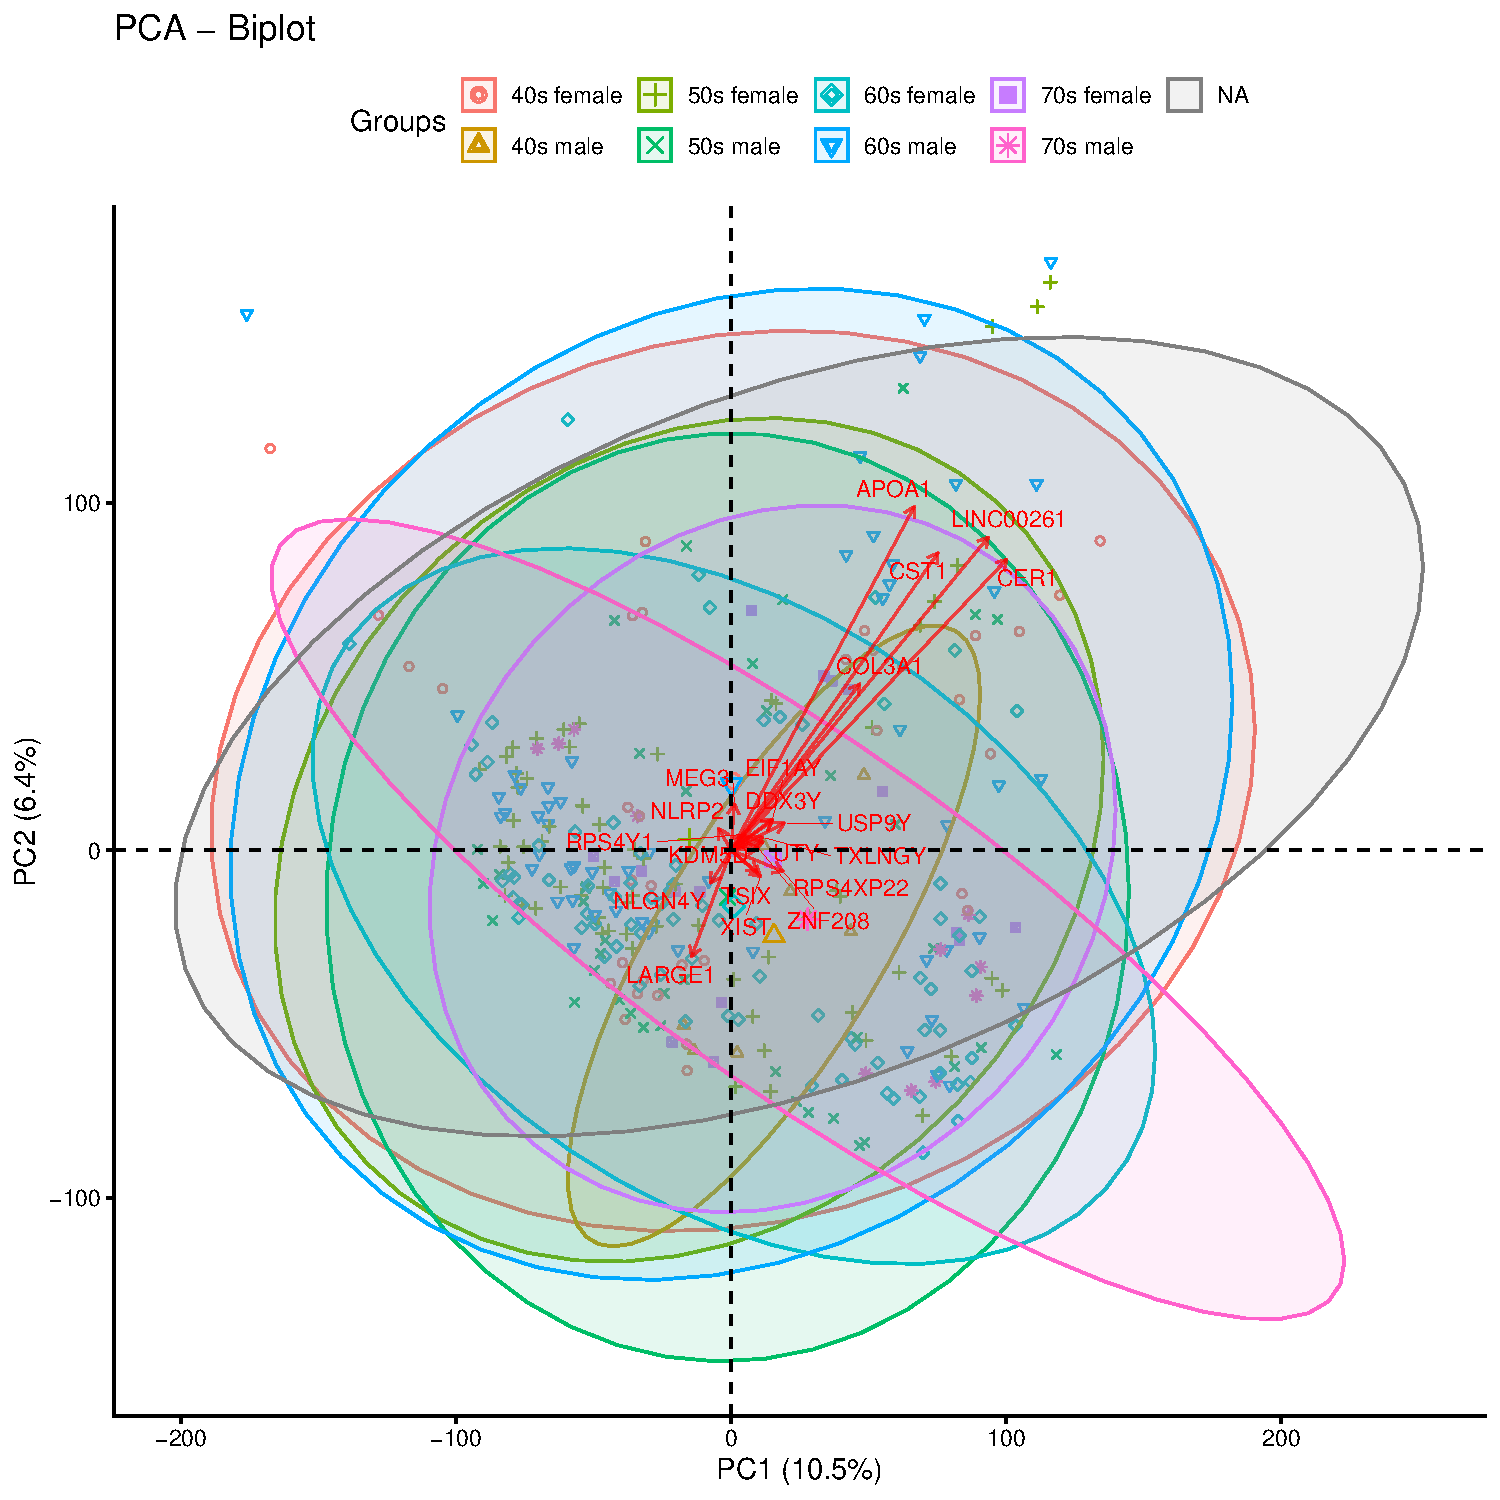
\includegraphics[keepaspectratio]{Final-Project-BIOL806_files/figure-pdf/fig-pca-sexage-1.pdf}}

}

\caption{\label{fig-pca-sexage}Caption.}

\end{figure}%

\begin{figure}

\centering{

\pandocbounded{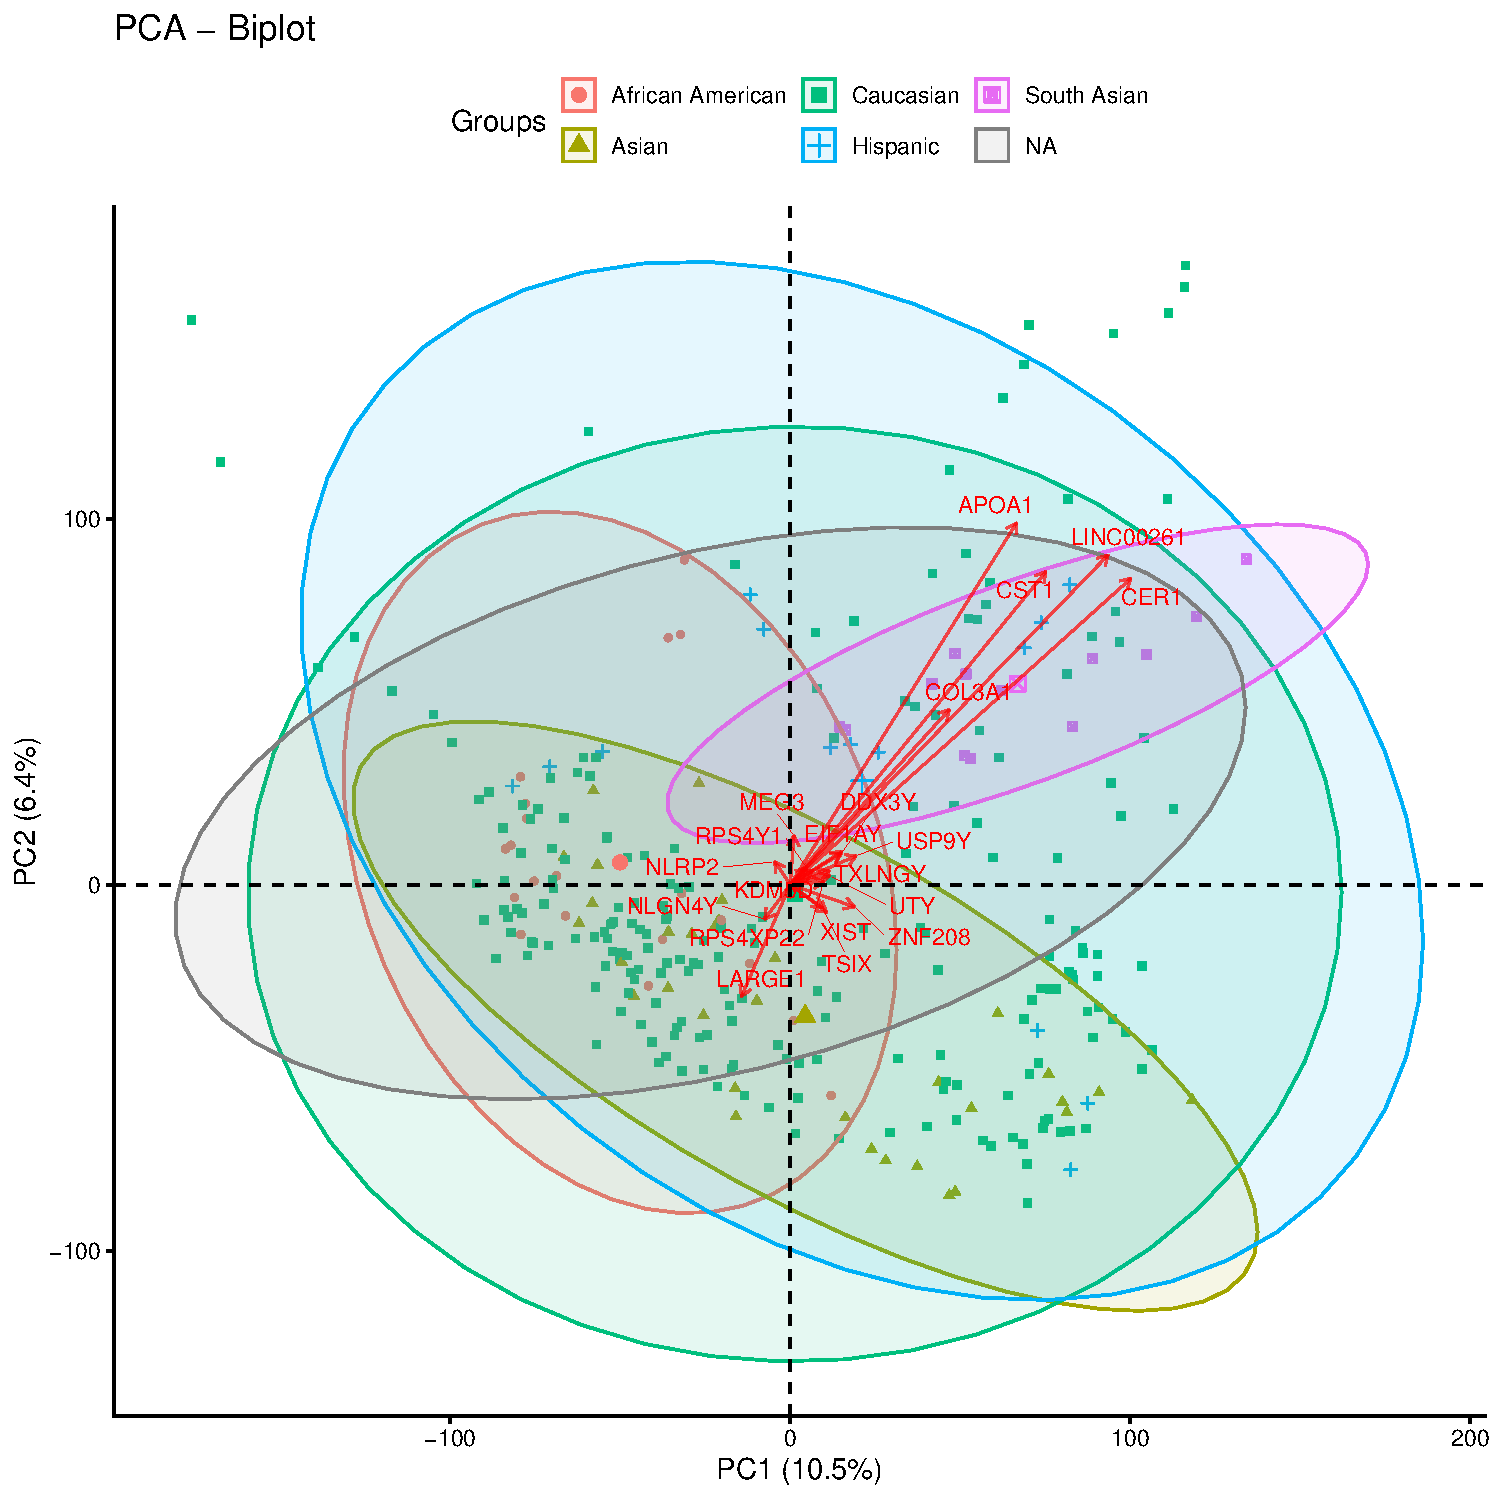
\includegraphics[keepaspectratio]{Final-Project-BIOL806_files/figure-pdf/fig-pca-race-1.pdf}}

}

\caption{\label{fig-pca-race}Caption.}

\end{figure}%

top 20 genes:

sex linked RPS4Y1 Ribosomal protein S4, Y-linked. Present only in males.
High variance indicates sex is a strong driver. XIST X-inactive specific
transcript. Expressed in females for X-chromosome inactivation.
Sex-linked. DDX3Y DEAD-box helicase, Y-linked. Male-specific. TSIX
Antisense of XIST, regulates X-chromosome inactivation. Female-specific.
TXLNGY Y-linked, involved in transcription/translation regulation. KDM5D
Lysine demethylase 5D, Y-linked. Male-specific. USP9Y Ubiquitin-specific
peptidase 9, Y-linked. Male-specific. EIF1AY Eukaryotic translation
initiation factor 1A, Y-linked. Male-specific. UTY Ubiquitously
transcribed tetratricopeptide repeat, Y-linked. Male-specific. NLGN4Y
Neuroligin 4, Y-linked. Male-specific. RPS4XP22 Pseudogene similar to
RPS4X/RPS4Y.

other genes CST1 Cystatin SN, extracellular protease inhibitor. May vary
in differentiation. CER1 Cerberus, secreted factor involved in early
development and differentiation. LARGE1 Glycosyltransferase, involved in
post-translational modification. NLRP2 NLR family pyrin domain
containing 2, involved in early development, oocyte/embryo regulation.
COL3A1 Collagen type III alpha 1, ECM protein, differentiation-related.
ZNF208 Zinc finger protein, transcription factor, potential regulatory
role. APOA1 Apolipoprotein A1, lipid transport, may reflect metabolic
differences. MEG3 Long non-coding RNA, tumor suppressor, epigenetic
regulation, differentiation-related. LINC00261 Long non-coding RNA,
involved in endoderm differentiation.

\subsubsection{Top 20 Genes}\label{top-20-genes}

\begin{figure}

\centering{

\pandocbounded{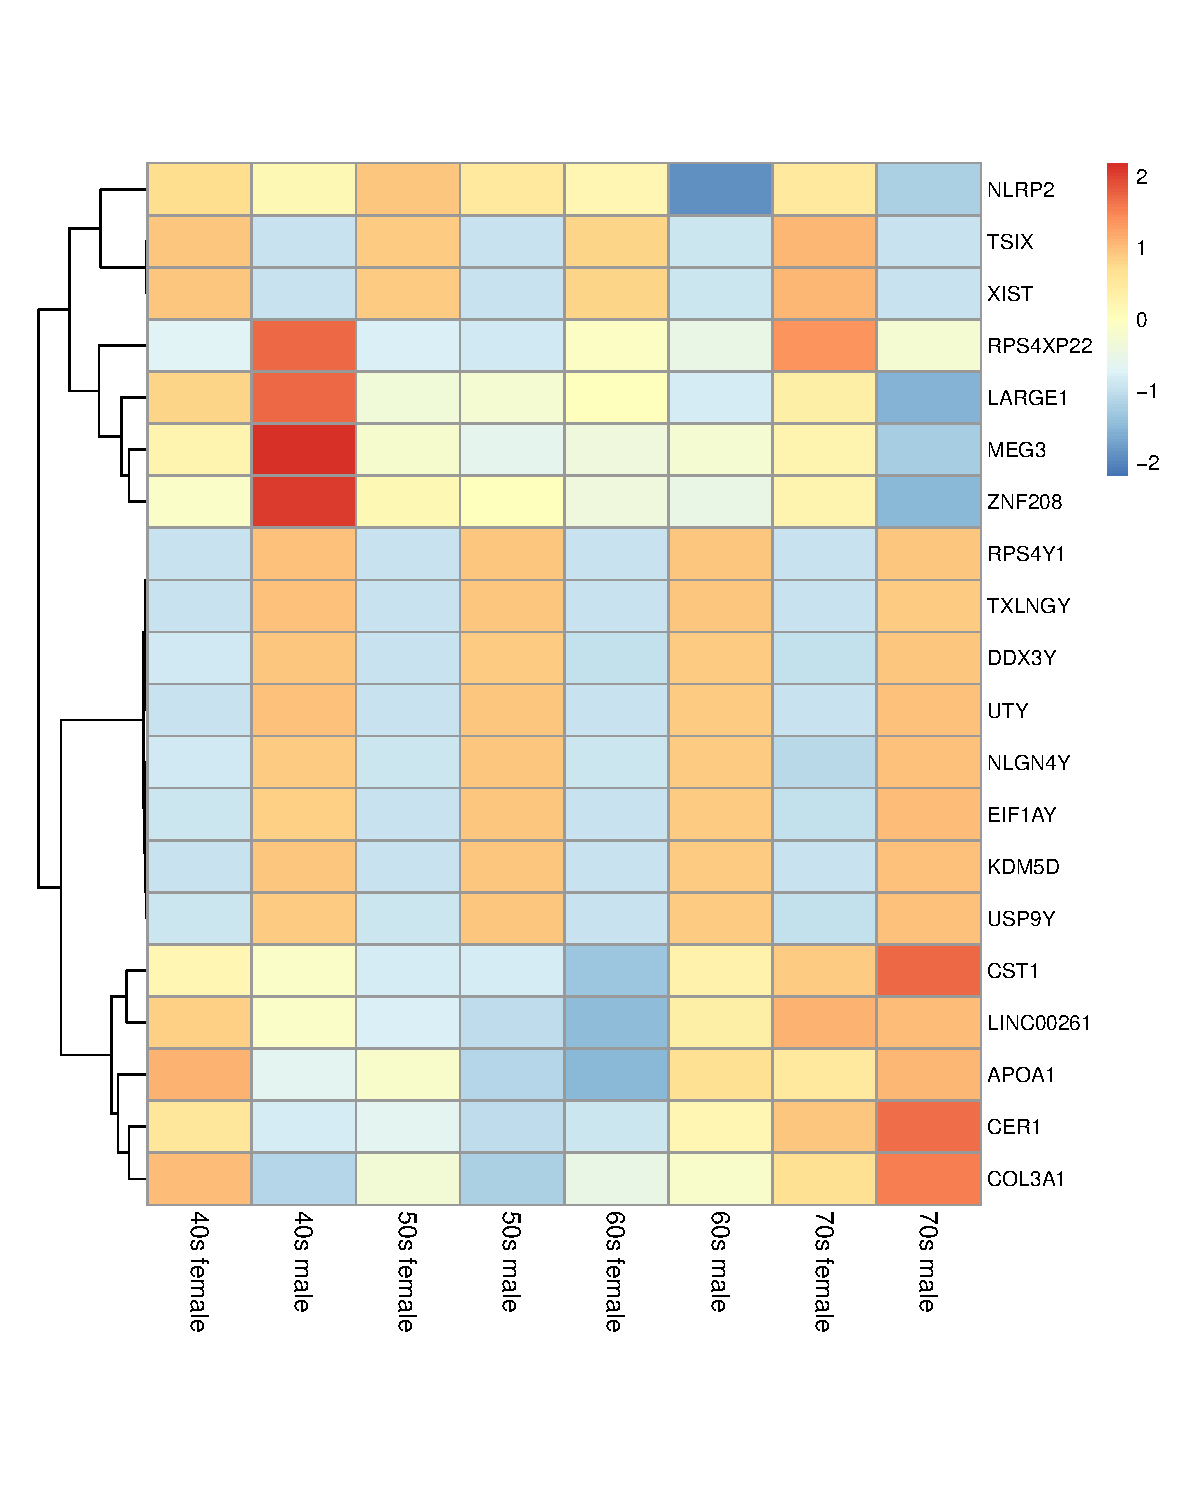
\includegraphics[keepaspectratio]{Final-Project-BIOL806_files/figure-pdf/fig-heatmap-top20-1.pdf}}

}

\caption{\label{fig-heatmap-top20}Expression of Genes with the Greatest
Variability}

\end{figure}%

\begin{figure}

\centering{

\pandocbounded{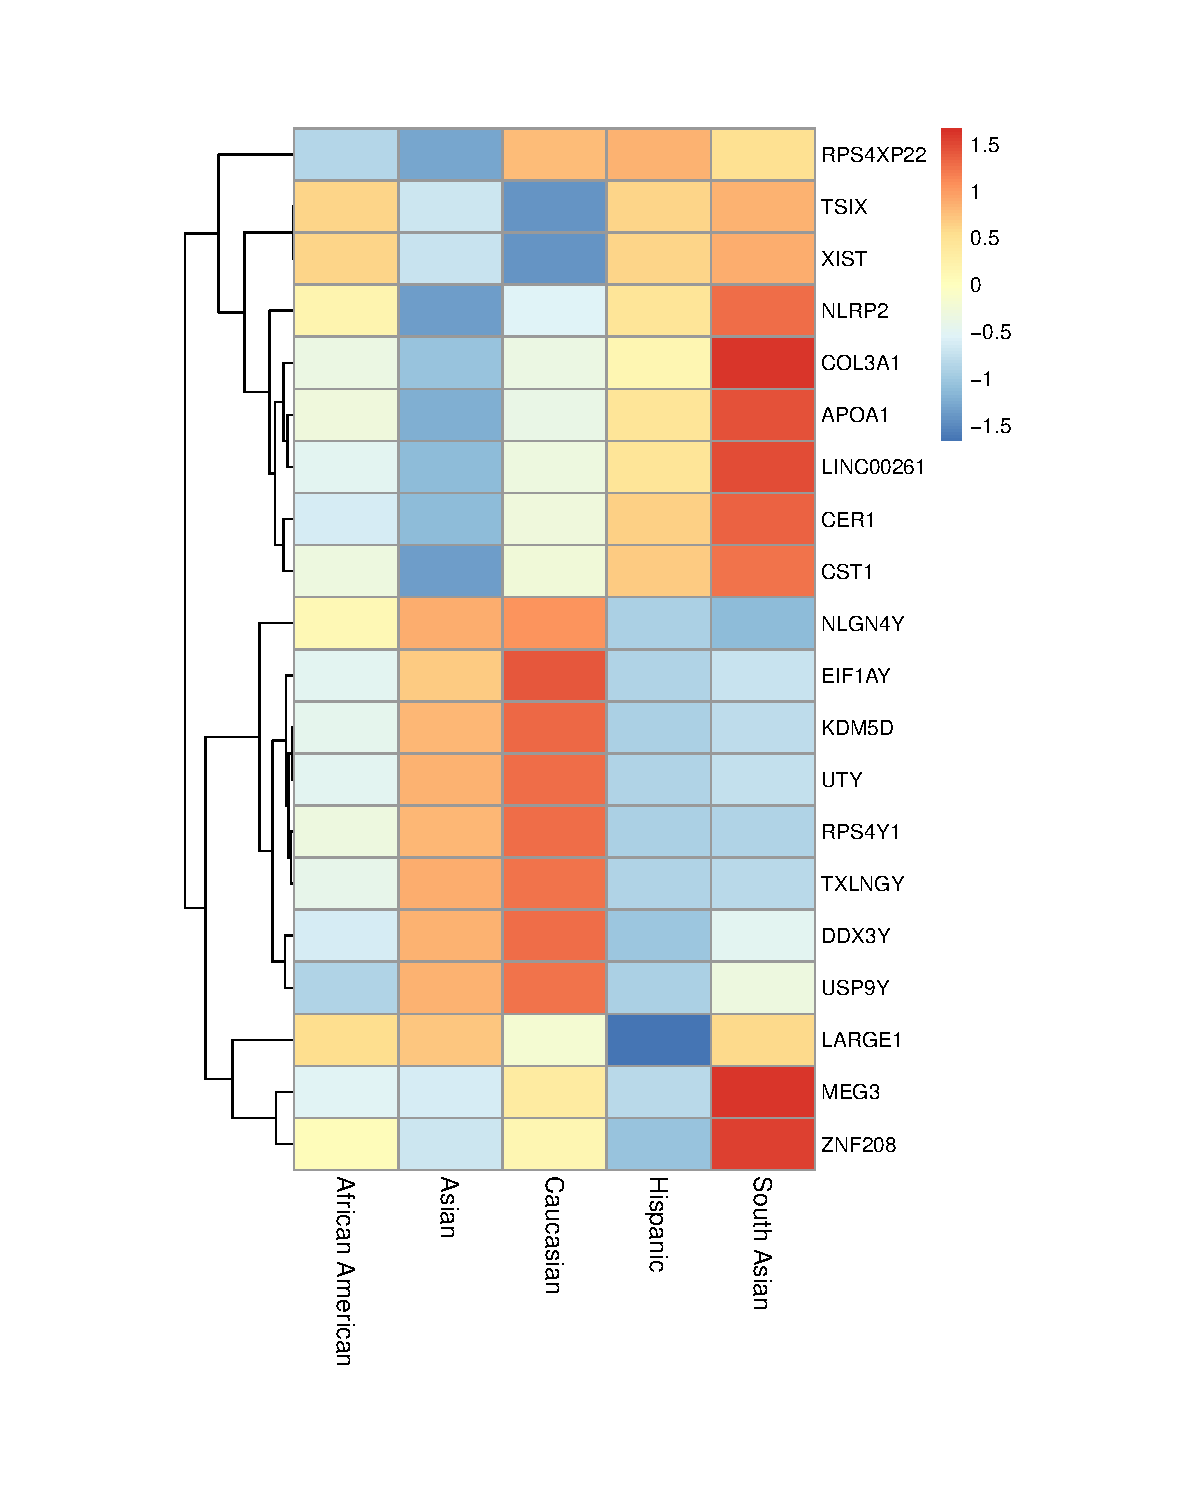
\includegraphics[keepaspectratio]{Final-Project-BIOL806_files/figure-pdf/fig-heatmap-top20-race-1.pdf}}

}

\caption{\label{fig-heatmap-top20-race}Expression of of Genes with the
Greatest Variability}

\end{figure}%

\subsubsection{Pluripotency Markers}\label{pluripotency-markers}

Expression of Pluripotency Genes (SOX2, POU5F1(OCT4), KLF4, MYC (c-Myc),
TRA-1-81 and 1-60 (PODXL), NANOG, FUT4 (SSEA4), LIN28A,alp

\begin{figure}

\centering{

\pandocbounded{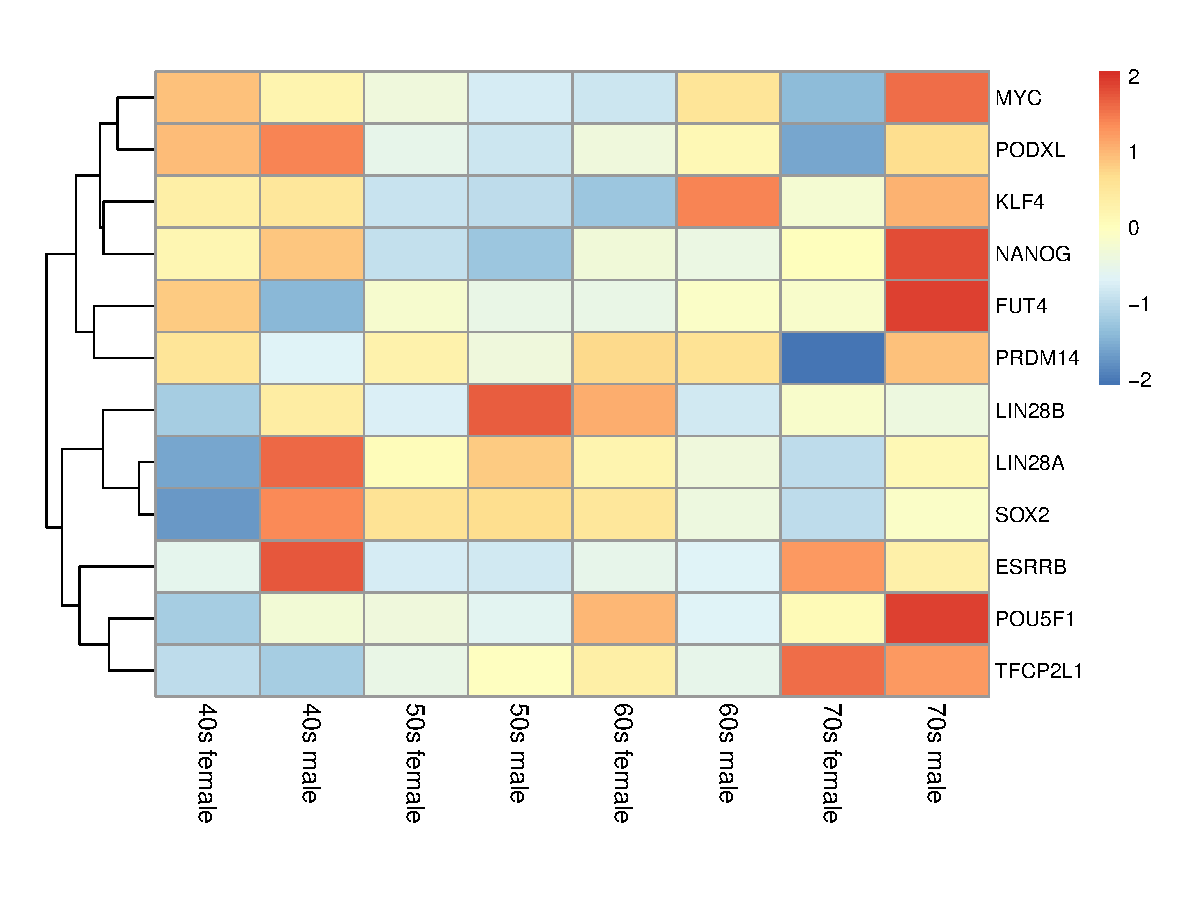
\includegraphics[keepaspectratio]{Final-Project-BIOL806_files/figure-pdf/fig-heatmap-pluripotency-1.pdf}}

}

\caption{\label{fig-heatmap-pluripotency}Expression of Pluripotency
Genes}

\end{figure}%

\begin{figure}

\centering{

\pandocbounded{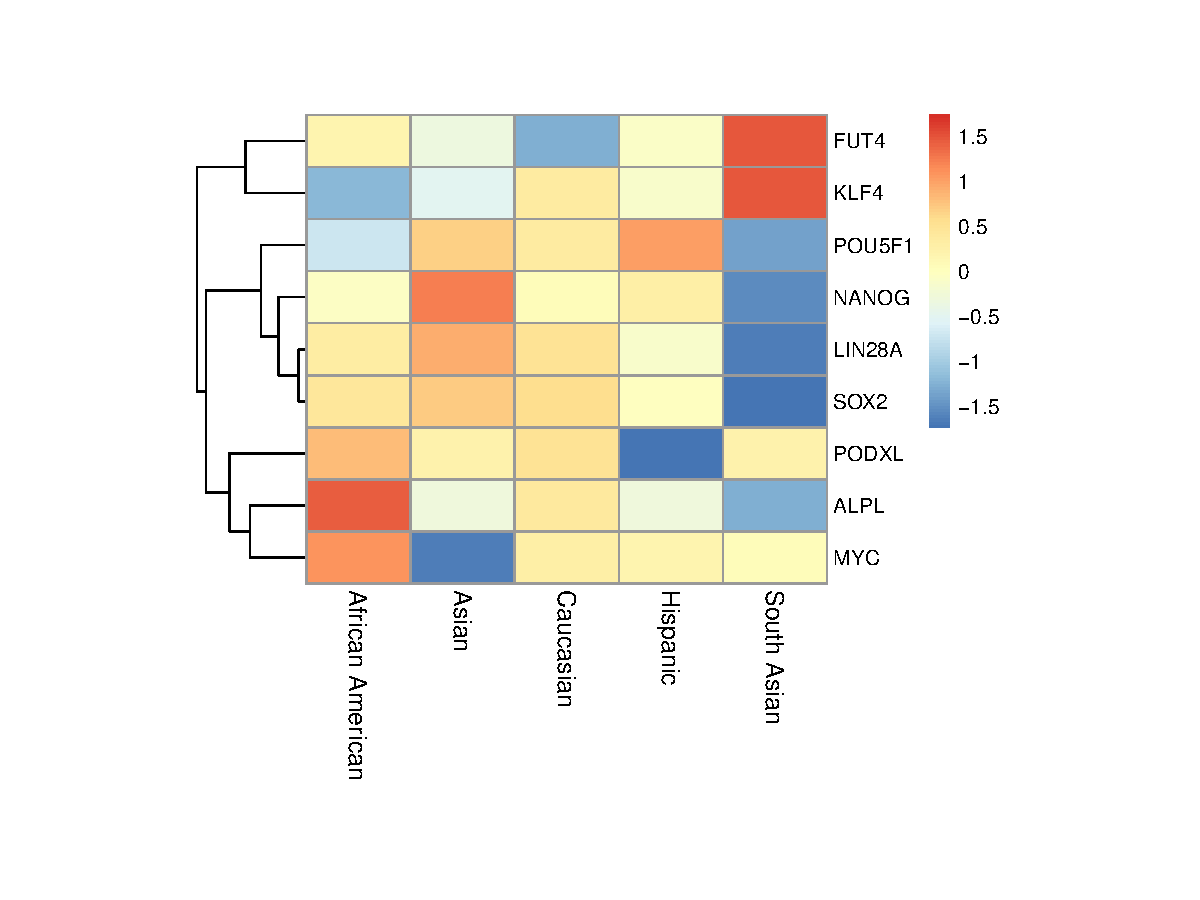
\includegraphics[keepaspectratio]{Final-Project-BIOL806_files/figure-pdf/fig-heatmap-pluripotency-race-1.pdf}}

}

\caption{\label{fig-heatmap-pluripotency-race}Expression of Pluripotency
Genes}

\end{figure}%

\begin{figure}

\centering{

\pandocbounded{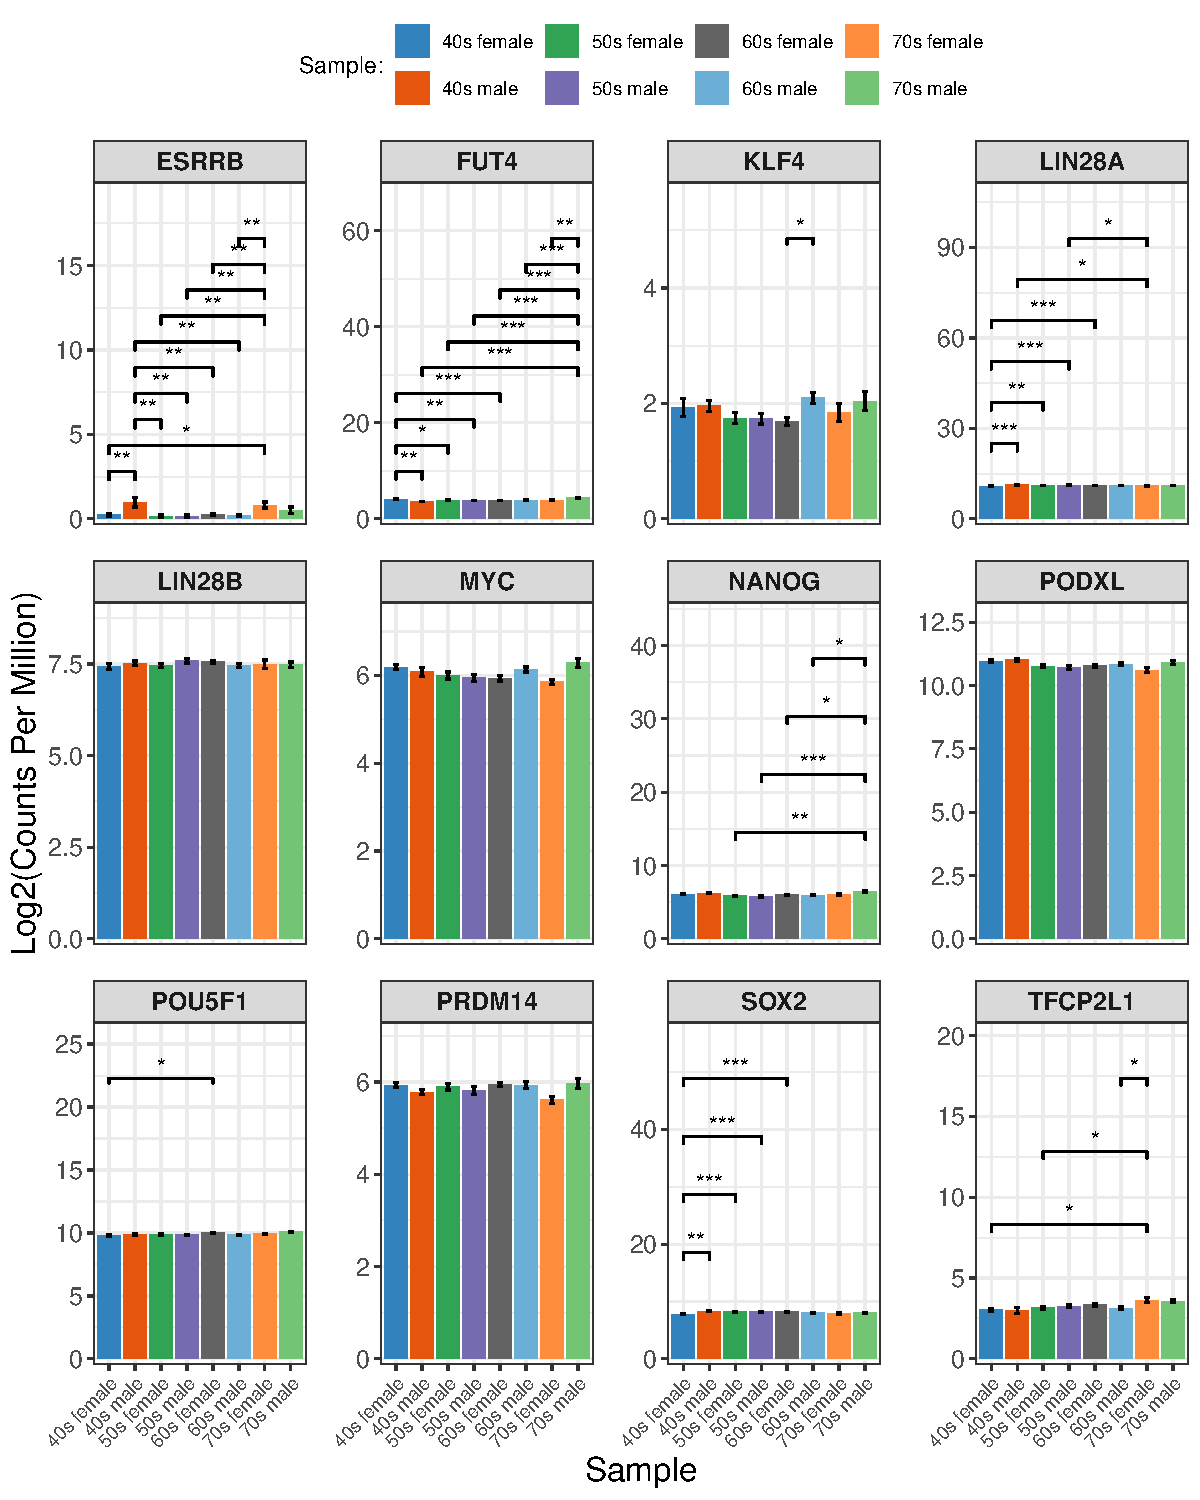
\includegraphics[keepaspectratio]{Final-Project-BIOL806_files/figure-pdf/fig-bargraph-pluripotency-1.pdf}}

}

\caption{\label{fig-bargraph-pluripotency}Expression of Pluripotency
Genes}

\end{figure}%

\begin{figure}

\centering{

\pandocbounded{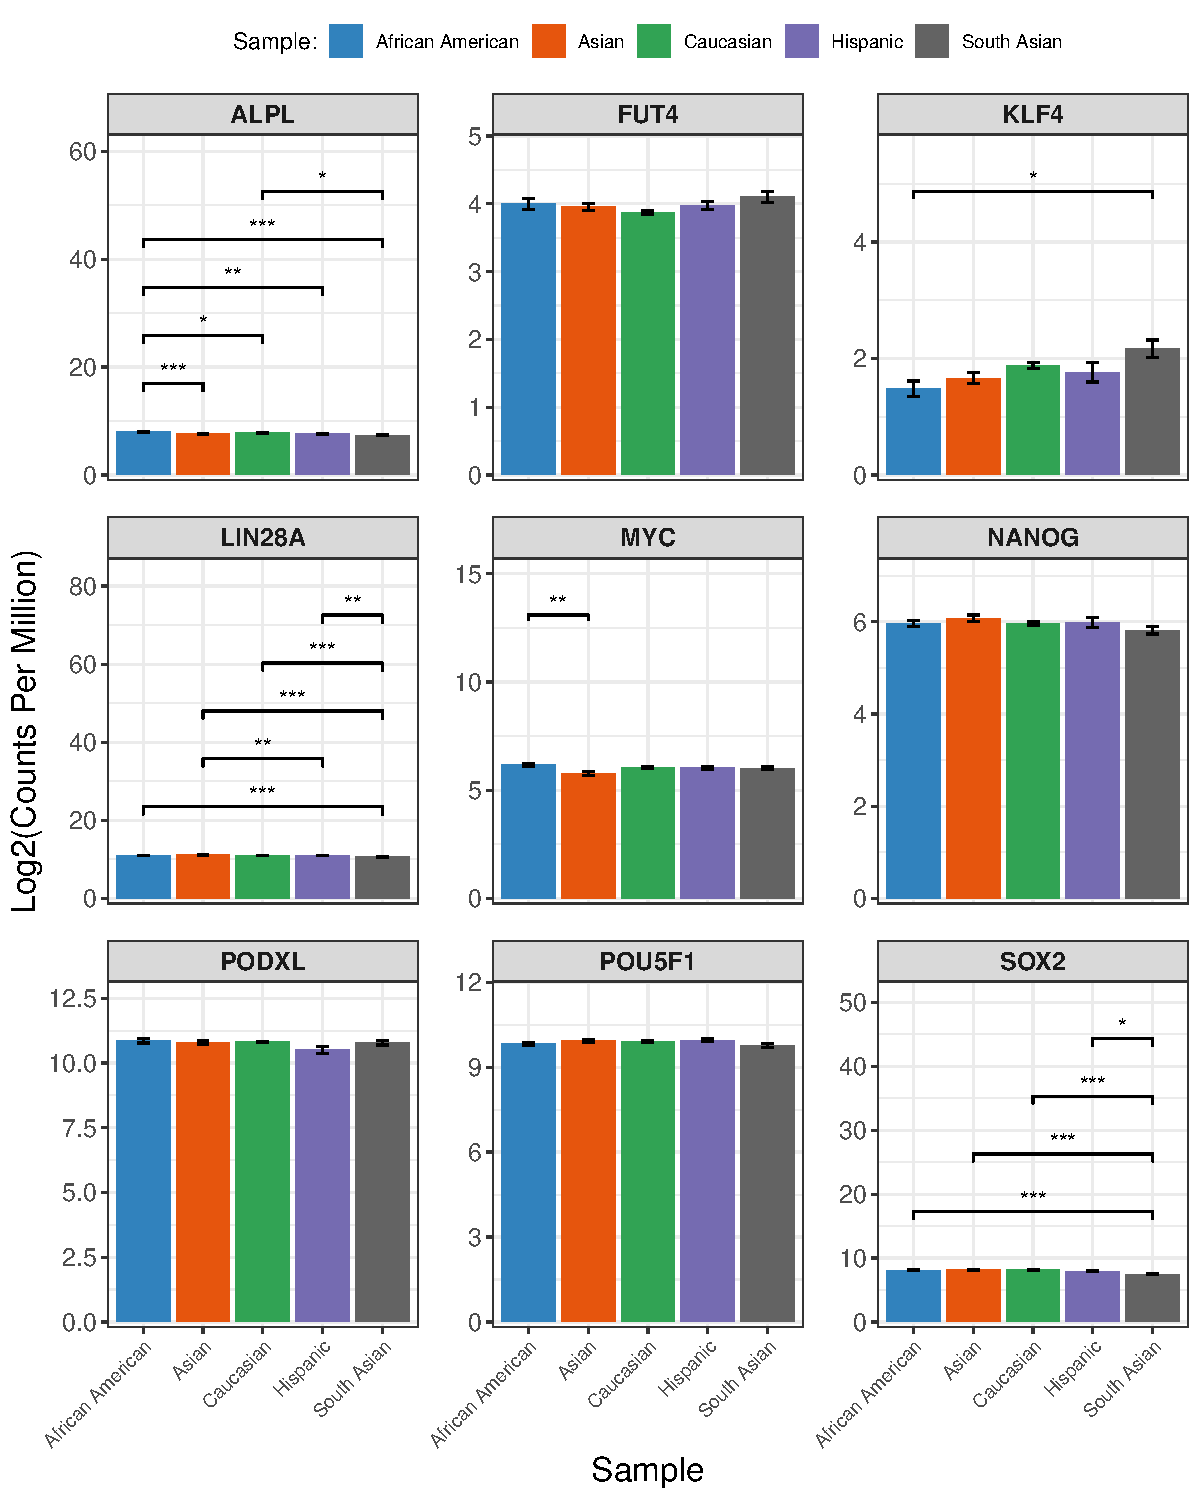
\includegraphics[keepaspectratio]{Final-Project-BIOL806_files/figure-pdf/fig-bargraph-pluripotency-race-1.pdf}}

}

\caption{\label{fig-bargraph-pluripotency-race}Expression of
Pluripotency Genes}

\end{figure}%

\emph{will remove lmm and qqplot outputs for final submission}

\begin{verbatim}
Linear mixed model fit by REML. t-tests use Satterthwaite's method [
lmerModLmerTest]
Formula: Expression ~ age_sex + (1 | `Gene name`)
   Data: df_pluri_agesex

REML criterion at convergence: 3193.4

Scaled residuals: 
    Min      1Q  Median      3Q     Max 
-4.9183 -0.5551  0.0387  0.5495  5.8829 

Random effects:
 Groups    Name        Variance Std.Dev.
 Gene name (Intercept) 9.8217   3.1340  
 Residual              0.1891   0.4349  
Number of obs: 2628, groups:  Gene name, 9

Fixed effects:
                    Estimate Std. Error         df t value Pr(>|t|)    
(Intercept)          7.27013    1.04498    8.00867   6.957 0.000117 ***
age_sex40s male      0.09329    0.05749 2612.00000   1.623 0.104766    
age_sex50s female   -0.02520    0.03180 2612.00000  -0.792 0.428209    
age_sex50s male     -0.04945    0.03508 2612.00000  -1.409 0.158846    
age_sex60s female   -0.02387    0.03108 2612.00000  -0.768 0.442562    
age_sex60s male      0.01372    0.03267 2612.00000   0.420 0.674581    
age_sex70s female   -0.09705    0.04668 2612.00000  -2.079 0.037703 *  
age_sex70s male      0.17852    0.05088 2612.00000   3.509 0.000458 ***
---
Signif. codes:  0 '***' 0.001 '**' 0.01 '*' 0.05 '.' 0.1 ' ' 1

Correlation of Fixed Effects:
            (Intr) ag_40m ag_50f ag_50m ag_60f ag_60m ag_70f
age_sx40sml -0.011                                          
ag_sx50sfml -0.020  0.371                                   
age_sx50sml -0.018  0.336  0.608                            
ag_sx60sfml -0.021  0.379  0.686  0.622                     
age_sx60sml -0.020  0.361  0.653  0.591  0.668              
ag_sx70sfml -0.014  0.253  0.457  0.414  0.467  0.445       
age_sx70sml -0.013  0.232  0.419  0.380  0.429  0.408  0.285
\end{verbatim}

\begin{verbatim}
Type III Analysis of Variance Table with Satterthwaite's method
        Sum Sq Mean Sq NumDF DenDF F value    Pr(>F)    
age_sex  6.331 0.90443     7  2612  4.7819 2.335e-05 ***
---
Signif. codes:  0 '***' 0.001 '**' 0.01 '*' 0.05 '.' 0.1 ' ' 1
\end{verbatim}

\begin{verbatim}
$emmeans
 age_sex    emmean   SE   df lower.CL upper.CL
 40s female   7.27 1.04 8.01     4.86     9.68
 40s male     7.36 1.05 8.04     4.95     9.77
 50s female   7.24 1.04 8.00     4.84     9.65
 50s male     7.22 1.04 8.01     4.81     9.63
 60s female   7.25 1.04 8.00     4.84     9.66
 60s male     7.28 1.04 8.00     4.87     9.69
 70s female   7.17 1.05 8.02     4.76     9.58
 70s male     7.45 1.05 8.03     5.04     9.86

Degrees-of-freedom method: kenward-roger 
Confidence level used: 0.95 

$contrasts
 contrast                estimate     SE   df t.ratio p.value
 40s female - 40s male   -0.09329 0.0575 2612  -1.623  0.7366
 40s female - 50s female  0.02520 0.0318 2612   0.792  0.9935
 40s female - 50s male    0.04945 0.0351 2612   1.409  0.8532
 40s female - 60s female  0.02387 0.0311 2612   0.768  0.9947
 40s female - 60s male   -0.01372 0.0327 2612  -0.420  0.9999
 40s female - 70s female  0.09705 0.0467 2612   2.079  0.4288
 40s female - 70s male   -0.17852 0.0509 2612  -3.509  0.0108
 40s male - 50s female    0.11849 0.0544 2612   2.178  0.3656
 40s male - 50s male      0.14273 0.0564 2612   2.531  0.1827
 40s male - 60s female    0.11715 0.0540 2612   2.170  0.3704
 40s male - 60s male      0.07957 0.0549 2612   1.449  0.8342
 40s male - 70s female    0.19034 0.0642 2612   2.963  0.0613
 40s male - 70s male     -0.08523 0.0674 2612  -1.265  0.9115
 50s female - 50s male    0.02425 0.0298 2612   0.814  0.9924
 50s female - 60s female -0.00133 0.0249 2612  -0.054  1.0000
 50s female - 60s male   -0.03892 0.0269 2612  -1.448  0.8348
 50s female - 70s female  0.07185 0.0428 2612   1.678  0.7020
 50s female - 70s male   -0.20372 0.0474 2612  -4.300  0.0005
 50s male - 60s female   -0.02558 0.0290 2612  -0.882  0.9877
 50s male - 60s male     -0.06316 0.0307 2612  -2.058  0.4429
 50s male - 70s female    0.04761 0.0453 2612   1.050  0.9665
 50s male - 70s male     -0.22797 0.0496 2612  -4.593  0.0001
 60s female - 60s male   -0.03758 0.0260 2612  -1.444  0.8364
 60s female - 70s female  0.07319 0.0423 2612   1.730  0.6673
 60s female - 70s male   -0.20239 0.0469 2612  -4.317  0.0004
 60s male - 70s female    0.11077 0.0435 2612   2.548  0.1760
 60s male - 70s male     -0.16480 0.0480 2612  -3.437  0.0139
 70s female - 70s male   -0.27557 0.0584 2612  -4.718  0.0001

Degrees-of-freedom method: kenward-roger 
P value adjustment: tukey method for comparing a family of 8 estimates 
\end{verbatim}

\begin{verbatim}
# A tibble: 18 x 6
   term    statistic parameter     p.value Gene        p_adj
   <chr>       <dbl>     <dbl>       <dbl> <chr>       <dbl>
 1 age_sex      2.06       7   0.0615      ALPL   0.0615    
 2 age_sex      2.06      60.4 0.0615      ALPL   0.0615    
 3 age_sex      9.07       7   0.000000127 LIN28A 0.00000114
 4 age_sex      9.07      60.9 0.000000127 LIN28A 0.00000114
 5 age_sex      5.72       7   0.0000453   SOX2   0.000136  
 6 age_sex      5.72      58.5 0.0000453   SOX2   0.000136  
 7 age_sex      4.27       7   0.000702    POU5F1 0.00105   
 8 age_sex      4.27      59.7 0.000702    POU5F1 0.00105   
 9 age_sex      3.66       7   0.00226     PODXL  0.00290   
10 age_sex      3.66      62.0 0.00226     PODXL  0.00290   
11 age_sex      4.47       7   0.000459    MYC    0.000827  
12 age_sex      4.47      60.5 0.000459    MYC    0.000827  
13 age_sex      2.53       7   0.0235      KLF4   0.0265    
14 age_sex      2.53      60.4 0.0235      KLF4   0.0265    
15 age_sex      8.14       7   0.000000748 FUT4   0.00000337
16 age_sex      8.14      57.4 0.000000748 FUT4   0.00000337
17 age_sex      4.87       7   0.000228    NANOG  0.000513  
18 age_sex      4.87      58.1 0.000228    NANOG  0.000513  
\end{verbatim}

\begin{verbatim}
NULL
\end{verbatim}

Residual variance = 0.2103 and intercept variance = 12.0276 means most
of the variation is between genes, not sex and age.

Fixed effects Sex effect (male): Expression is slightly higher in males,
for all genes, by 0.036 logCPM; significant at p = 0.0205, but only at
0.03648 units (log2 count per million/relative expression?).

Age effects: Only the 70s group is significantly higher than 40s (p =
0.0135), 0.08018 units. 50s and 60s are not significantly different from
40s.

Type III Analysis of Variance Table with Satterthwaite's method -
confirms both sex and age\_decade have a significant effect on
pluripotency gene expression when averaged across all genes.

Predicted mean logCPM expression (adjusted means, not raw means)

female: 6.20. male: 6.23

40s: 6.20, 50s: 6.18, 60s: 6.21, 70s: 6.28

Overall, pluripotency gene expression is slightly higher in males
compared to females, regardless of age. Expression also shows an
increasing trend with age, with samples from individuals in their 70s
being significantly higher than those from individuals in their 40s.
Differences between other age decades (50s, 60s) and 40s were not
statistically significant.

\begin{Shaded}
\begin{Highlighting}[]
\CommentTok{\#pluripotency genes, race stats }

\NormalTok{df\_pluri\_race }\OtherTok{\textless{}{-}}\NormalTok{ pluri\_race\_results}\SpecialCharTok{$}\NormalTok{data}
 \CommentTok{\# Fit mixed model}
\CommentTok{\#model the response variable, Expression, for the fixed effects, age and sex}
\CommentTok{\# genes are treated as a random effect, all with different y intercepts,}
\CommentTok{\# since expression levels vary by gene}
\NormalTok{lmm\_pluri\_race }\OtherTok{\textless{}{-}} \FunctionTok{lmer}\NormalTok{(Expression }\SpecialCharTok{\textasciitilde{}}\NormalTok{ race }\SpecialCharTok{+}\NormalTok{ (}\DecValTok{1} \SpecialCharTok{|} \StringTok{\textasciigrave{}}\AttributeTok{Gene name}\StringTok{\textasciigrave{}}\NormalTok{), }\AttributeTok{data =}\NormalTok{ df\_pluri\_race)}
\NormalTok{summary\_pluri\_race }\OtherTok{\textless{}{-}} \FunctionTok{summary}\NormalTok{(lmm\_pluri\_race)}
  \CommentTok{\# type III ANOVA to test significance of fixed effects on expression}
\NormalTok{lmm\_pluri\_race\_anova }\OtherTok{\textless{}{-}} \FunctionTok{anova}\NormalTok{(lmm\_pluri\_race, }\AttributeTok{type =} \DecValTok{3}\NormalTok{)}

\CommentTok{\# estimated marginal means (or least{-}squares means) with pairwise comparisons}
\NormalTok{lmm\_pluri\_race\_emm }\OtherTok{\textless{}{-}} \FunctionTok{emmeans}\NormalTok{(lmm\_pluri\_race, pairwise }\SpecialCharTok{\textasciitilde{}}\NormalTok{ race)}

\CommentTok{\#lmm summary}
\NormalTok{summary\_pluri\_race}
\end{Highlighting}
\end{Shaded}

\begin{verbatim}
Linear mixed model fit by REML. t-tests use Satterthwaite's method [
lmerModLmerTest]
Formula: Expression ~ race + (1 | `Gene name`)
   Data: df_pluri_race

REML criterion at convergence: 3194

Scaled residuals: 
    Min      1Q  Median      3Q     Max 
-4.8788 -0.5462  0.0551  0.5406  5.7992 

Random effects:
 Groups    Name        Variance Std.Dev.
 Gene name (Intercept) 9.8217   3.134   
 Residual              0.1901   0.436   
Number of obs: 2628, groups:  Gene name, 9

Fixed effects:
                  Estimate Std. Error         df t value Pr(>|t|)    
(Intercept)      7.270e+00  1.045e+00  8.015e+00   6.956 0.000117 ***
raceAsian       -3.734e-02  4.118e-02  2.615e+03  -0.907 0.364633    
raceCaucasian    4.469e-03  3.400e-02  2.615e+03   0.131 0.895432    
raceHispanic    -7.695e-02  5.064e-02  2.615e+03  -1.519 0.128778    
raceSouth Asian -1.426e-01  5.178e-02  2.615e+03  -2.754 0.005932 ** 
---
Signif. codes:  0 '***' 0.001 '**' 0.01 '*' 0.05 '.' 0.1 ' ' 1

Correlation of Fixed Effects:
            (Intr) racAsn rcCcsn rcHspn
raceAsian   -0.025                     
raceCaucasn -0.030  0.754              
raceHispanc -0.020  0.506  0.613       
raceSothAsn -0.020  0.495  0.600  0.403
\end{verbatim}

\begin{Shaded}
\begin{Highlighting}[]
\CommentTok{\#anova}
\NormalTok{lmm\_pluri\_race\_anova}
\end{Highlighting}
\end{Shaded}

\begin{verbatim}
Type III Analysis of Variance Table with Satterthwaite's method
     Sum Sq Mean Sq NumDF DenDF F value   Pr(>F)   
race 3.2581 0.81453     4  2615  4.2849 0.001856 **
---
Signif. codes:  0 '***' 0.001 '**' 0.01 '*' 0.05 '.' 0.1 ' ' 1
\end{verbatim}

\begin{Shaded}
\begin{Highlighting}[]
\CommentTok{\#means }
\NormalTok{lmm\_pluri\_race\_emm}
\end{Highlighting}
\end{Shaded}

\begin{verbatim}
$emmeans
 race             emmean   SE   df lower.CL upper.CL
 African American   7.27 1.05 8.01     4.86     9.68
 Asian              7.23 1.04 8.01     4.82     9.64
 Caucasian          7.27 1.04 8.00     4.87     9.68
 Hispanic           7.19 1.05 8.02     4.78     9.60
 South Asian        7.13 1.05 8.02     4.72     9.54

Degrees-of-freedom method: kenward-roger 
Confidence level used: 0.95 

$contrasts
 contrast                       estimate     SE   df t.ratio p.value
 African American - Asian        0.03734 0.0412 2615   0.907  0.8944
 African American - Caucasian   -0.00447 0.0340 2615  -0.131  0.9999
 African American - Hispanic     0.07695 0.0506 2615   1.519  0.5498
 African American - South Asian  0.14258 0.0518 2615   2.754  0.0468
 Asian - Caucasian              -0.04181 0.0272 2615  -1.537  0.5381
 Asian - Hispanic                0.03961 0.0464 2615   0.854  0.9133
 Asian - South Asian             0.10524 0.0476 2615   2.211  0.1757
 Caucasian - Hispanic            0.08142 0.0401 2615   2.030  0.2518
 Caucasian - South Asian         0.14705 0.0415 2615   3.541  0.0037
 Hispanic - South Asian          0.06563 0.0560 2615   1.173  0.7672

Degrees-of-freedom method: kenward-roger 
P value adjustment: tukey method for comparing a family of 5 estimates 
\end{verbatim}

\begin{Shaded}
\begin{Highlighting}[]
\CommentTok{\#gene anova FDR corrected }
\NormalTok{pluri\_race\_results}\SpecialCharTok{$}\NormalTok{anova\_fdr}
\end{Highlighting}
\end{Shaded}

\begin{verbatim}
# A tibble: 18 x 6
   term  statistic parameter     p.value Gene        p_adj
   <chr>     <dbl>     <dbl>       <dbl> <chr>       <dbl>
 1 race       8.57       4   0.0000462   ALPL   0.000139  
 2 race       8.57      38.9 0.0000462   ALPL   0.000139  
 3 race      13.7        4   0.000000366 LIN28A 0.00000330
 4 race      13.7       40.5 0.000000366 LIN28A 0.00000330
 5 race       9.79       4   0.0000154   SOX2   0.0000695 
 6 race       9.79      37.8 0.0000154   SOX2   0.0000695 
 7 race       2.12       4   0.0967      POU5F1 0.124     
 8 race       2.12      39.5 0.0967      POU5F1 0.124     
 9 race       1.36       4   0.268       PODXL  0.268     
10 race       1.36      37.9 0.268       PODXL  0.268     
11 race       2.99       4   0.0288      MYC    0.0518    
12 race       2.99      44.2 0.0288      MYC    0.0518    
13 race       3.93       4   0.00906     KLF4   0.0204    
14 race       3.93      38.5 0.00906     KLF4   0.0204    
15 race       2.50       4   0.0579      FUT4   0.0869    
16 race       2.50      39.0 0.0579      FUT4   0.0869    
17 race       1.62       4   0.188       NANOG  0.211     
18 race       1.62      40.8 0.188       NANOG  0.211     
\end{verbatim}

\begin{Shaded}
\begin{Highlighting}[]
\CommentTok{\#gene tueky corrected}
\NormalTok{pluri\_race\_results}\SpecialCharTok{$}\NormalTok{tukey\_fdr}
\end{Highlighting}
\end{Shaded}

\begin{verbatim}
NULL
\end{verbatim}

\subsubsection{Differentiation Markers}\label{differentiation-markers}

Expression of Differentiation Genes (ectoderm: PAX6, NESTIN (NES)
(neural projenitor/stem cell markers), KRT14 (epithelial), endoderm:
SOX17, AFP (hepatic), PDX1 (pancreatic), mesoderm: CD34 (hematopoitic),
CD90 (THY1)(mesenchymal), NKX2.5 (cardiac progenitor)).

\begin{figure}

\centering{

\pandocbounded{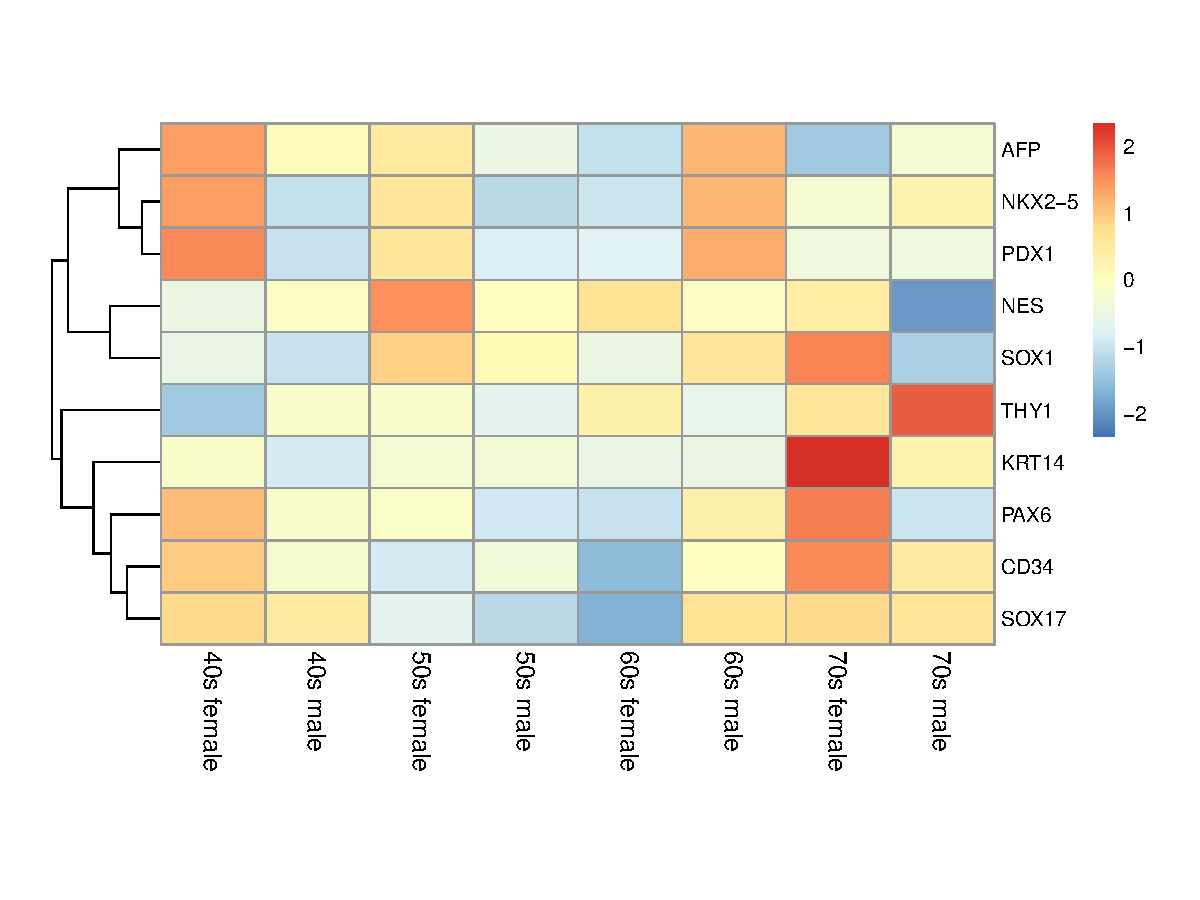
\includegraphics[keepaspectratio]{Final-Project-BIOL806_files/figure-pdf/fig-heatmap-diff-1.pdf}}

}

\caption{\label{fig-heatmap-diff}Expression of Differentiation Genes}

\end{figure}%

\begin{figure}

\centering{

\pandocbounded{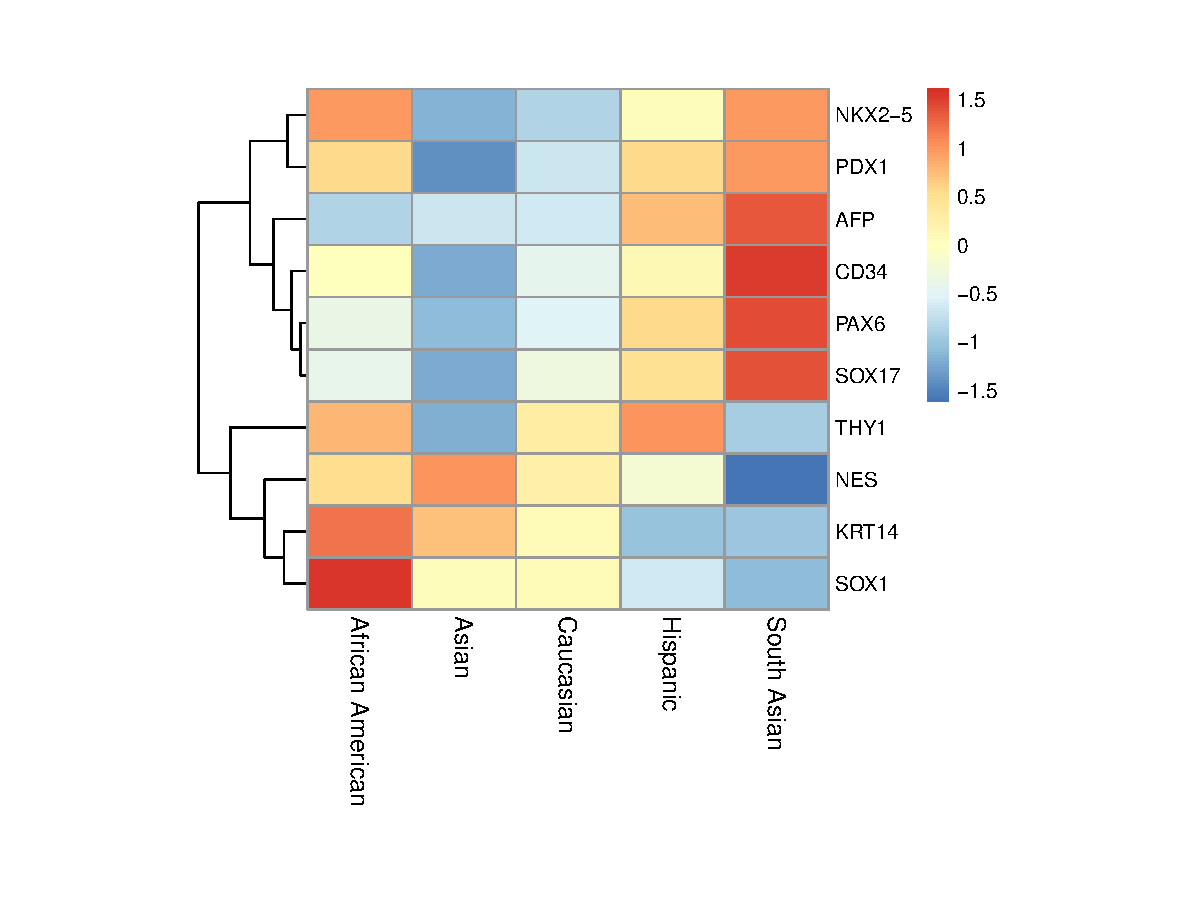
\includegraphics[keepaspectratio]{Final-Project-BIOL806_files/figure-pdf/fig-heatmap-diff-race-1.pdf}}

}

\caption{\label{fig-heatmap-diff-race}Expression of Differentiation
Genes}

\end{figure}%

\begin{figure}

\centering{

\pandocbounded{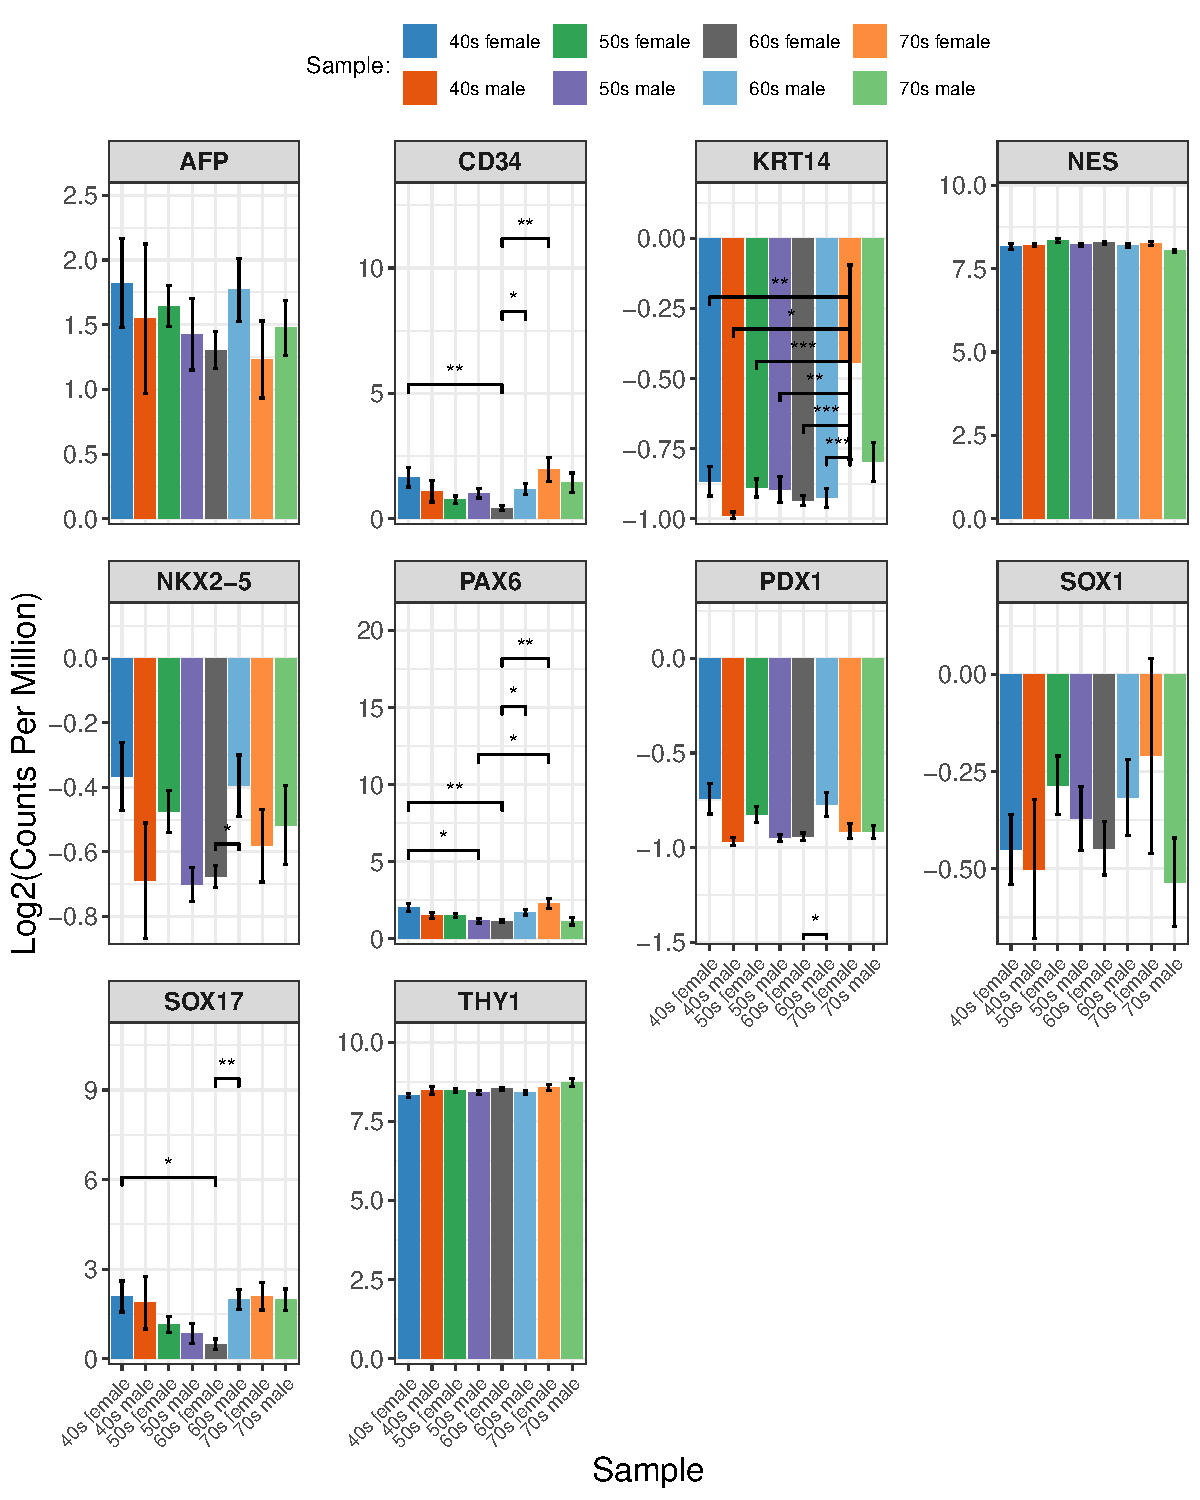
\includegraphics[keepaspectratio]{Final-Project-BIOL806_files/figure-pdf/fig-bargraph-diff-1.pdf}}

}

\caption{\label{fig-bargraph-diff}Expression of Differentiation Genes}

\end{figure}%

\begin{figure}

\centering{

\pandocbounded{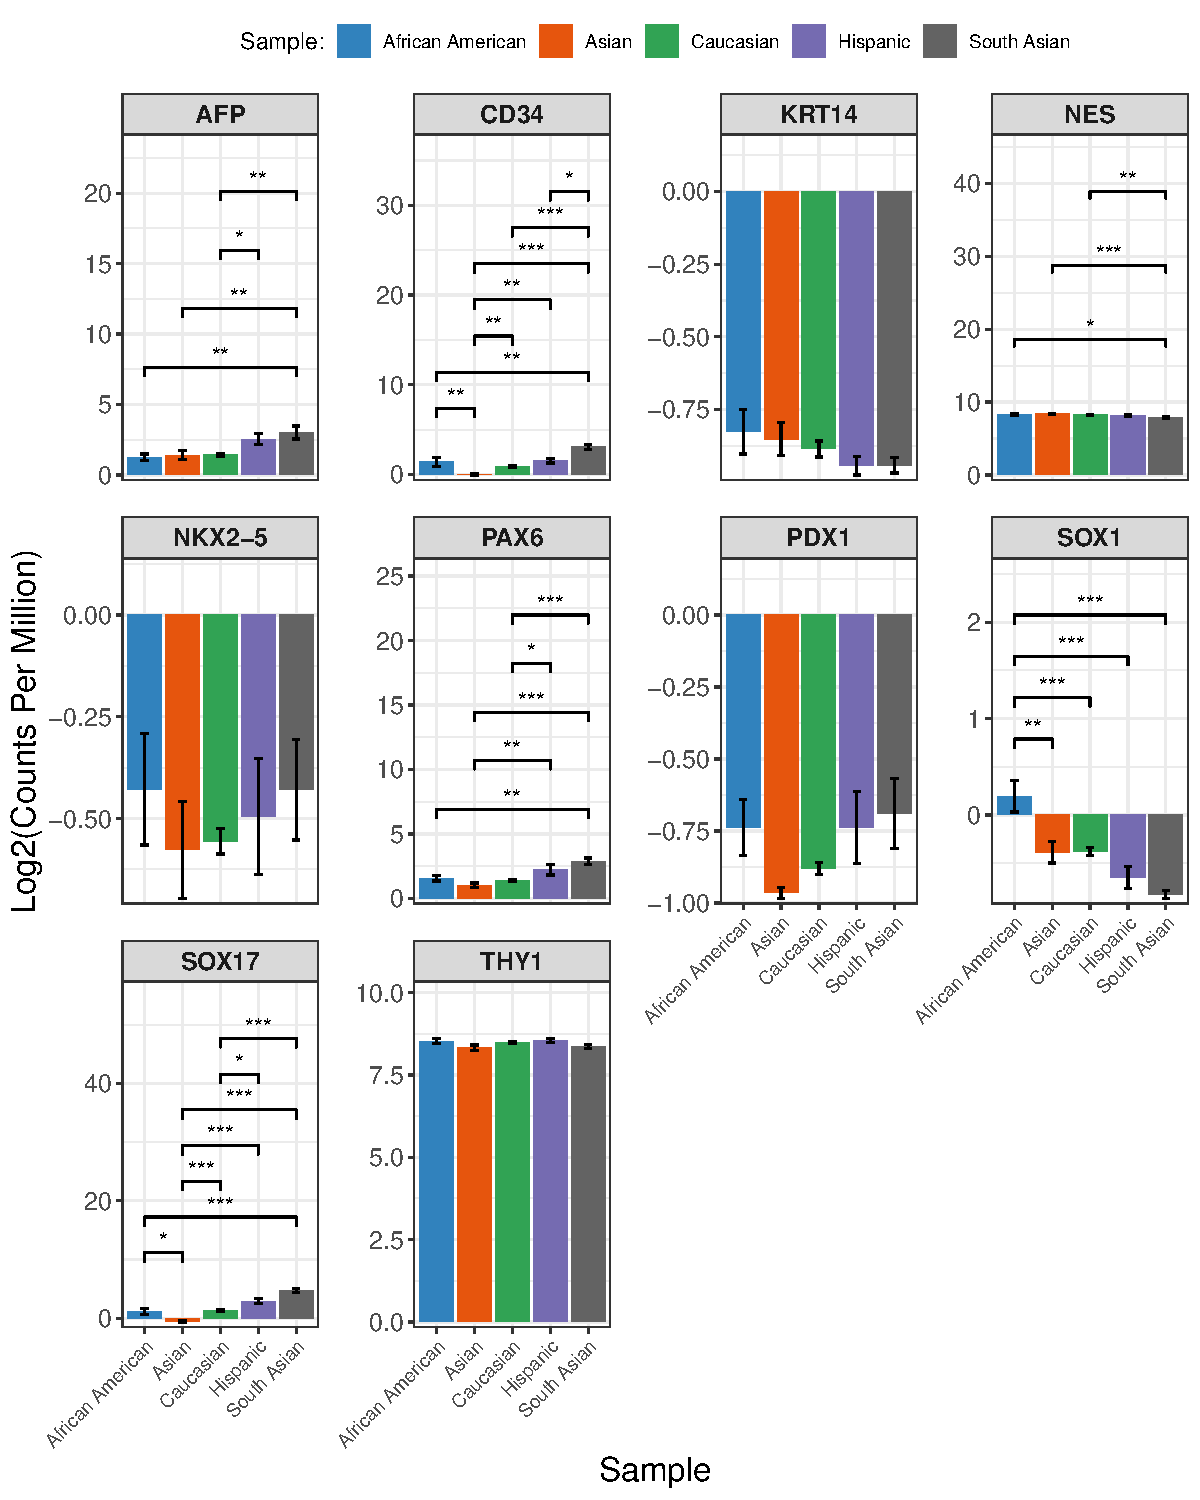
\includegraphics[keepaspectratio]{Final-Project-BIOL806_files/figure-pdf/fig-bargraph-diff-race-1.pdf}}

}

\caption{\label{fig-bargraph-diff-race}Expression of Differentiation
Genes}

\end{figure}%

\begin{verbatim}
Linear mixed model fit by REML. t-tests use Satterthwaite's method [
lmerModLmerTest]
Formula: Expression ~ age_sex + (1 | `Gene name`)
   Data: df_diff_agesex

REML criterion at convergence: 8009.8

Scaled residuals: 
    Min      1Q  Median      3Q     Max 
-2.5706 -0.4198 -0.0940  0.2866  6.9085 

Random effects:
 Groups    Name        Variance Std.Dev.
 Gene name (Intercept) 13.168   3.629   
 Residual               1.195   1.093   
Number of obs: 2628, groups:  Gene name, 9

Fixed effects:
                    Estimate Std. Error         df t value Pr(>|t|)    
(Intercept)          2.45694    1.21138    8.04192   2.028 0.076886 .  
age_sex40s male     -0.22896    0.14447 2612.00000  -1.585 0.113140    
age_sex50s female   -0.26888    0.07993 2612.00000  -3.364 0.000779 ***
age_sex50s male     -0.39756    0.08817 2612.00000  -4.509 6.80e-06 ***
age_sex60s female   -0.50038    0.07810 2612.00000  -6.407 1.76e-10 ***
age_sex60s male     -0.10258    0.08209 2612.00000  -1.250 0.211573    
age_sex70s female    0.03669    0.11731 2612.00000   0.313 0.754522    
age_sex70s male     -0.17168    0.12786 2612.00000  -1.343 0.179475    
---
Signif. codes:  0 '***' 0.001 '**' 0.01 '*' 0.05 '.' 0.1 ' ' 1

Correlation of Fixed Effects:
            (Intr) ag_40m ag_50f ag_50m ag_60f ag_60m ag_70f
age_sx40sml -0.024                                          
ag_sx50sfml -0.044  0.371                                   
age_sx50sml -0.040  0.336  0.608                            
ag_sx60sfml -0.045  0.379  0.686  0.622                     
age_sx60sml -0.043  0.361  0.653  0.591  0.668              
ag_sx70sfml -0.030  0.253  0.457  0.414  0.467  0.445       
age_sx70sml -0.028  0.232  0.419  0.380  0.429  0.408  0.285
\end{verbatim}

\begin{verbatim}
Type III Analysis of Variance Table with Satterthwaite's method
        Sum Sq Mean Sq NumDF DenDF F value    Pr(>F)    
age_sex 87.255  12.465     7  2612  10.435 5.527e-13 ***
---
Signif. codes:  0 '***' 0.001 '**' 0.01 '*' 0.05 '.' 0.1 ' ' 1
\end{verbatim}

\begin{verbatim}
$emmeans
 age_sex    emmean   SE   df lower.CL upper.CL
 40s female   2.46 1.21 8.04   -0.334     5.25
 40s male     2.23 1.22 8.18   -0.567     5.02
 50s female   2.19 1.21 8.02   -0.602     4.98
 50s male     2.06 1.21 8.03   -0.731     4.85
 60s female   1.96 1.21 8.01   -0.834     4.75
 60s male     2.35 1.21 8.02   -0.436     5.14
 70s female   2.49 1.21 8.10   -0.299     5.29
 70s male     2.29 1.21 8.13   -0.508     5.08

Degrees-of-freedom method: kenward-roger 
Confidence level used: 0.95 

$contrasts
 contrast                estimate     SE   df t.ratio p.value
 40s female - 40s male     0.2290 0.1440 2612   1.585  0.7596
 40s female - 50s female   0.2689 0.0799 2612   3.364  0.0177
 40s female - 50s male     0.3976 0.0882 2612   4.509  0.0002
 40s female - 60s female   0.5004 0.0781 2612   6.407  <.0001
 40s female - 60s male     0.1026 0.0821 2612   1.250  0.9168
 40s female - 70s female  -0.0367 0.1170 2612  -0.313  1.0000
 40s female - 70s male     0.1717 0.1280 2612   1.343  0.8824
 40s male - 50s female     0.0399 0.1370 2612   0.292  1.0000
 40s male - 50s male       0.1686 0.1420 2612   1.190  0.9350
 40s male - 60s female     0.2714 0.1360 2612   2.000  0.4817
 40s male - 60s male      -0.1264 0.1380 2612  -0.916  0.9846
 40s male - 70s female    -0.2656 0.1610 2612  -1.645  0.7226
 40s male - 70s male      -0.0573 0.1690 2612  -0.338  1.0000
 50s female - 50s male     0.1287 0.0748 2612   1.720  0.6744
 50s female - 60s female   0.2315 0.0626 2612   3.695  0.0055
 50s female - 60s male    -0.1663 0.0676 2612  -2.461  0.2127
 50s female - 70s female  -0.3056 0.1080 2612  -2.839  0.0861
 50s female - 70s male    -0.0972 0.1190 2612  -0.816  0.9922
 50s male - 60s female     0.1028 0.0729 2612   1.411  0.8525
 50s male - 60s male      -0.2950 0.0771 2612  -3.824  0.0034
 50s male - 70s female    -0.4342 0.1140 2612  -3.812  0.0035
 50s male - 70s male      -0.2259 0.1250 2612  -1.811  0.6127
 60s female - 60s male    -0.3978 0.0654 2612  -6.083  <.0001
 60s female - 70s female  -0.5371 0.1060 2612  -5.053  <.0001
 60s female - 70s male    -0.3287 0.1180 2612  -2.790  0.0980
 60s male - 70s female    -0.1393 0.1090 2612  -1.275  0.9083
 60s male - 70s male       0.0691 0.1210 2612   0.573  0.9992
 70s female - 70s male     0.2084 0.1470 2612   1.419  0.8485

Degrees-of-freedom method: kenward-roger 
P value adjustment: tukey method for comparing a family of 8 estimates 
\end{verbatim}

\begin{verbatim}
# A tibble: 18 x 6
   term    statistic parameter  p.value Gene     p_adj
   <chr>       <dbl>     <dbl>    <dbl> <chr>    <dbl>
 1 age_sex     3.64        7   0.00224  NES    0.00505
 2 age_sex     3.64       65.6 0.00224  NES    0.00505
 3 age_sex     4.36        7   0.000671 CD34   0.00302
 4 age_sex     4.36       54.4 0.000671 CD34   0.00302
 5 age_sex     0.768       7   0.616    AFP    0.616  
 6 age_sex     0.768      57.8 0.616    AFP    0.616  
 7 age_sex     3.00        7   0.00965  NKX2-5 0.0124 
 8 age_sex     3.00       55.0 0.00965  NKX2-5 0.0124 
 9 age_sex     4.62        7   0.000391 SOX17  0.00302
10 age_sex     4.62       56.3 0.000391 SOX17  0.00302
11 age_sex     4.01        7   0.00124  PAX6   0.00371
12 age_sex     4.01       57.2 0.00124  PAX6   0.00371
13 age_sex     1.88        7   0.0894   THY1   0.101  
14 age_sex     1.88       56.4 0.0894   THY1   0.101  
15 age_sex     2.98        7   0.00897  PDX1   0.0124 
16 age_sex     2.98       64.5 0.00897  PDX1   0.0124 
17 age_sex     3.42        7   0.00338  KRT14  0.00609
18 age_sex     3.42       69.8 0.00338  KRT14  0.00609
\end{verbatim}

\begin{verbatim}
NULL
\end{verbatim}

\begin{Shaded}
\begin{Highlighting}[]
\CommentTok{\#diff genes, race stats }

\NormalTok{df\_diff\_race }\OtherTok{\textless{}{-}}\NormalTok{ diff\_race\_results}\SpecialCharTok{$}\NormalTok{data}
 \CommentTok{\# Fit mixed model}
\CommentTok{\#model the response variable, Expression, for the fixed effects, age and sex}
\CommentTok{\# genes are treated as a random effect, all with different y intercepts,}
\CommentTok{\# since expression levels vary by gene}
\NormalTok{lmm\_diff\_race }\OtherTok{\textless{}{-}} \FunctionTok{lmer}\NormalTok{(Expression }\SpecialCharTok{\textasciitilde{}}\NormalTok{ race }\SpecialCharTok{+}\NormalTok{ (}\DecValTok{1} \SpecialCharTok{|} \StringTok{\textasciigrave{}}\AttributeTok{Gene name}\StringTok{\textasciigrave{}}\NormalTok{), }\AttributeTok{data =}\NormalTok{ df\_diff\_race)}
\NormalTok{summary\_diff\_race }\OtherTok{\textless{}{-}} \FunctionTok{summary}\NormalTok{(lmm\_diff\_race)}
  \CommentTok{\# type III ANOVA to test significance of fixed effects on expression}
\NormalTok{lmm\_diff\_race\_anova }\OtherTok{\textless{}{-}} \FunctionTok{anova}\NormalTok{(lmm\_diff\_race, }\AttributeTok{type =} \DecValTok{3}\NormalTok{)}

\CommentTok{\# estimated marginal means (or least{-}squares means) with pairwise comparisons}
\NormalTok{lmm\_diff\_race\_emm }\OtherTok{\textless{}{-}} \FunctionTok{emmeans}\NormalTok{(lmm\_diff\_race, pairwise }\SpecialCharTok{\textasciitilde{}}\NormalTok{ race)}

\CommentTok{\#lmm summary}
\NormalTok{summary\_diff\_race}
\end{Highlighting}
\end{Shaded}

\begin{verbatim}
Linear mixed model fit by REML. t-tests use Satterthwaite's method [
lmerModLmerTest]
Formula: Expression ~ race + (1 | `Gene name`)
   Data: df_diff_race

REML criterion at convergence: 7933

Scaled residuals: 
    Min      1Q  Median      3Q     Max 
-2.3319 -0.4624 -0.0815  0.2796  7.1792 

Random effects:
 Groups    Name        Variance Std.Dev.
 Gene name (Intercept) 13.169   3.629   
 Residual               1.163   1.078   
Number of obs: 2628, groups:  Gene name, 9

Fixed effects:
                  Estimate Std. Error         df t value Pr(>|t|)    
(Intercept)        2.23968    1.21228    8.06596   1.847  0.10157    
raceAsian         -0.42975    0.10187 2615.00000  -4.218 2.54e-05 ***
raceCaucasian     -0.07731    0.08409 2615.00000  -0.919  0.35798    
raceHispanic       0.39902    0.12527 2615.00000   3.185  0.00146 ** 
raceSouth Asian    0.85435    0.12808 2615.00000   6.671 3.10e-11 ***
---
Signif. codes:  0 '***' 0.001 '**' 0.01 '*' 0.05 '.' 0.1 ' ' 1

Correlation of Fixed Effects:
            (Intr) racAsn rcCcsn rcHspn
raceAsian   -0.052                     
raceCaucasn -0.063  0.754              
raceHispanc -0.043  0.506  0.613       
raceSothAsn -0.042  0.495  0.600  0.403
\end{verbatim}

\begin{Shaded}
\begin{Highlighting}[]
\CommentTok{\#anova}
\NormalTok{lmm\_diff\_race\_anova}
\end{Highlighting}
\end{Shaded}

\begin{verbatim}
Type III Analysis of Variance Table with Satterthwaite's method
     Sum Sq Mean Sq NumDF DenDF F value    Pr(>F)    
race 165.78  41.445     4  2615  35.632 < 2.2e-16 ***
---
Signif. codes:  0 '***' 0.001 '**' 0.01 '*' 0.05 '.' 0.1 ' ' 1
\end{verbatim}

\begin{Shaded}
\begin{Highlighting}[]
\CommentTok{\#means }
\NormalTok{lmm\_diff\_race\_emm}
\end{Highlighting}
\end{Shaded}

\begin{verbatim}
$emmeans
 race             emmean   SE   df lower.CL upper.CL
 African American   2.24 1.21 8.07   -0.552     5.03
 Asian              1.81 1.21 8.04   -0.981     4.60
 Caucasian          2.16 1.21 8.00   -0.627     4.95
 Hispanic           2.64 1.21 8.10   -0.154     5.43
 South Asian        3.09 1.21 8.10    0.301     5.89

Degrees-of-freedom method: kenward-roger 
Confidence level used: 0.95 

$contrasts
 contrast                       estimate     SE   df t.ratio p.value
 African American - Asian         0.4297 0.1020 2615   4.218  0.0002
 African American - Caucasian     0.0773 0.0841 2615   0.919  0.8895
 African American - Hispanic     -0.3990 0.1250 2615  -3.185  0.0127
 African American - South Asian  -0.8544 0.1280 2615  -6.671  <.0001
 Asian - Caucasian               -0.3524 0.0673 2615  -5.239  <.0001
 Asian - Hispanic                -0.8288 0.1150 2615  -7.228  <.0001
 Asian - South Asian             -1.2841 0.1180 2615 -10.908  <.0001
 Caucasian - Hispanic            -0.4763 0.0992 2615  -4.802  <.0001
 Caucasian - South Asian         -0.9317 0.1030 2615  -9.070  <.0001
 Hispanic - South Asian          -0.4553 0.1380 2615  -3.288  0.0090

Degrees-of-freedom method: kenward-roger 
P value adjustment: tukey method for comparing a family of 5 estimates 
\end{verbatim}

\begin{Shaded}
\begin{Highlighting}[]
\CommentTok{\#gene anova FDR corrected }
\NormalTok{diff\_race\_results}\SpecialCharTok{$}\NormalTok{anova\_fdr}
\end{Highlighting}
\end{Shaded}

\begin{verbatim}
# A tibble: 18 x 6
   term  statistic parameter  p.value Gene      p_adj
   <chr>     <dbl>     <dbl>    <dbl> <chr>     <dbl>
 1 race      4.40        4   5.16e- 3 NES    7.98e- 3
 2 race      4.40       37.4 5.16e- 3 NES    7.98e- 3
 3 race     37.4         4   7.78e-13 CD34   3.50e-12
 4 race     37.4        38.9 7.78e-13 CD34   3.50e-12
 5 race      4.78        4   3.28e- 3 AFP    7.39e- 3
 6 race      4.78       36.9 3.28e- 3 AFP    7.39e- 3
 7 race      0.452       4   7.70e- 1 NKX2-5 7.70e- 1
 8 race      0.452      36.0 7.70e- 1 NKX2-5 7.70e- 1
 9 race     62.0         4   1.74e-16 SOX17  1.57e-15
10 race     62.0        39.5 1.74e-16 SOX17  1.57e-15
11 race      8.92        4   3.91e- 5 PAX6   1.17e- 4
12 race      8.92       36.7 3.91e- 5 PAX6   1.17e- 4
13 race      2.35        4   6.96e- 2 THY1   8.95e- 2
14 race      2.35       41.9 6.96e- 2 THY1   8.95e- 2
15 race      4.38        4   5.32e- 3 PDX1   7.98e- 3
16 race      4.38       37.1 5.32e- 3 PDX1   7.98e- 3
17 race      1.35        4   2.66e- 1 KRT14  2.99e- 1
18 race      1.35       50.5 2.66e- 1 KRT14  2.99e- 1
\end{verbatim}

\begin{Shaded}
\begin{Highlighting}[]
\CommentTok{\#gene tueky corrected}
\NormalTok{diff\_race\_results}\SpecialCharTok{$}\NormalTok{tukey\_fdr}
\end{Highlighting}
\end{Shaded}

\begin{verbatim}
NULL
\end{verbatim}

\subsubsection{Housekeeping Genes}\label{housekeeping-genes}

Figure 5. Expression of Housekeeping Genes (some sort of general figure
or sorted by housekeeping type (i.e.~ribosomal, metabolic, cytoskeleton,
etc.))

\begin{figure}

\centering{

\pandocbounded{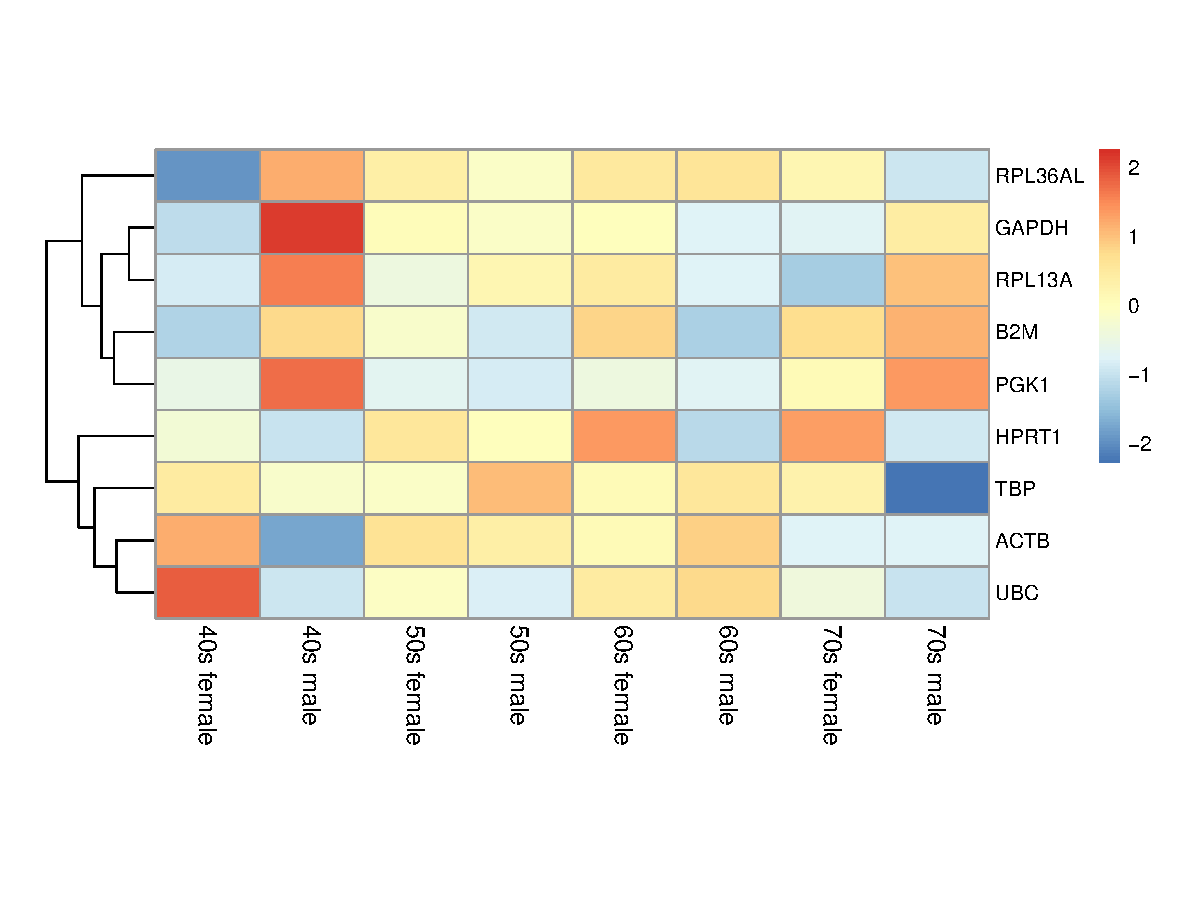
\includegraphics[keepaspectratio]{Final-Project-BIOL806_files/figure-pdf/fig-heatmap-hk-1.pdf}}

}

\caption{\label{fig-heatmap-hk}Expression of Housekeeping Genes}

\end{figure}%

\begin{figure}

\centering{

\pandocbounded{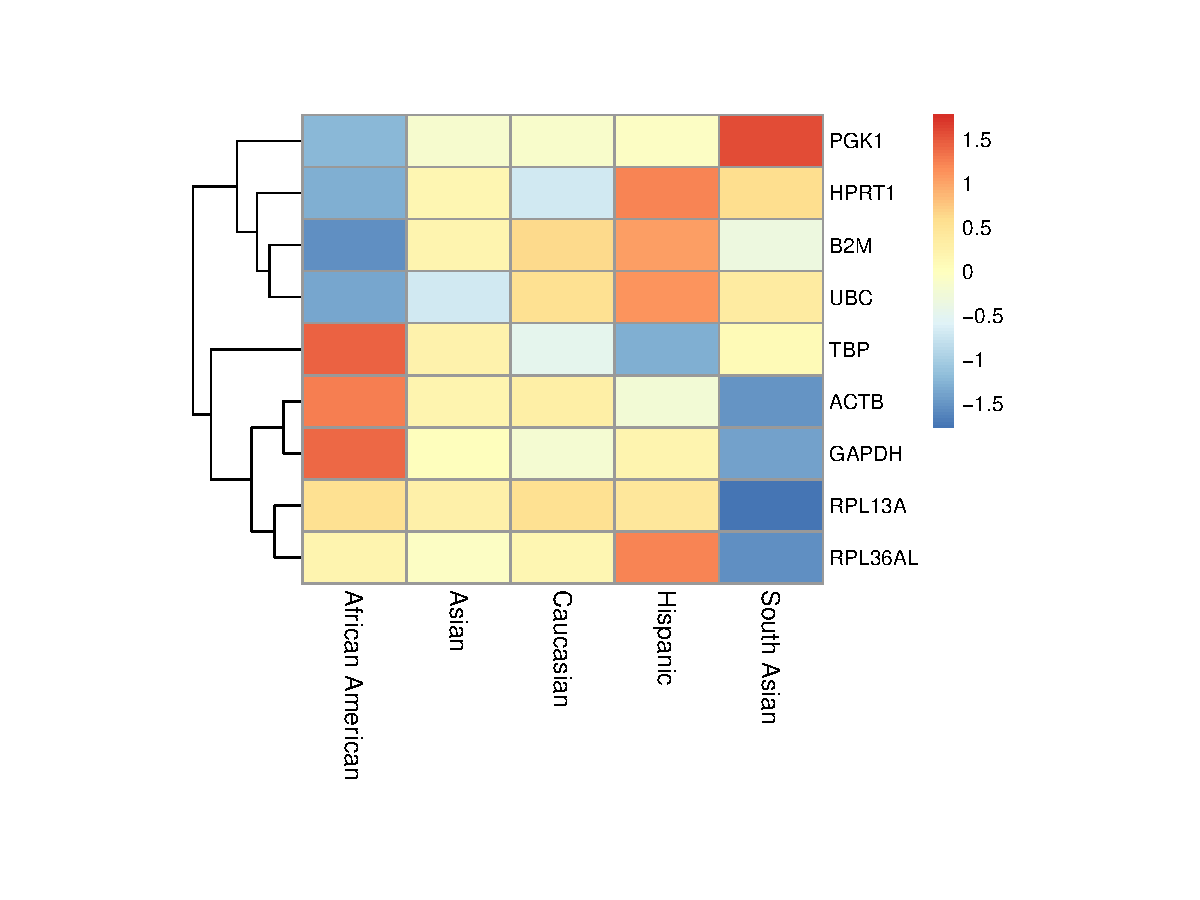
\includegraphics[keepaspectratio]{Final-Project-BIOL806_files/figure-pdf/fig-heatmap-hk-race-1.pdf}}

}

\caption{\label{fig-heatmap-hk-race}Expression of Housekeeping Genes}

\end{figure}%

\begin{figure}

\centering{

\pandocbounded{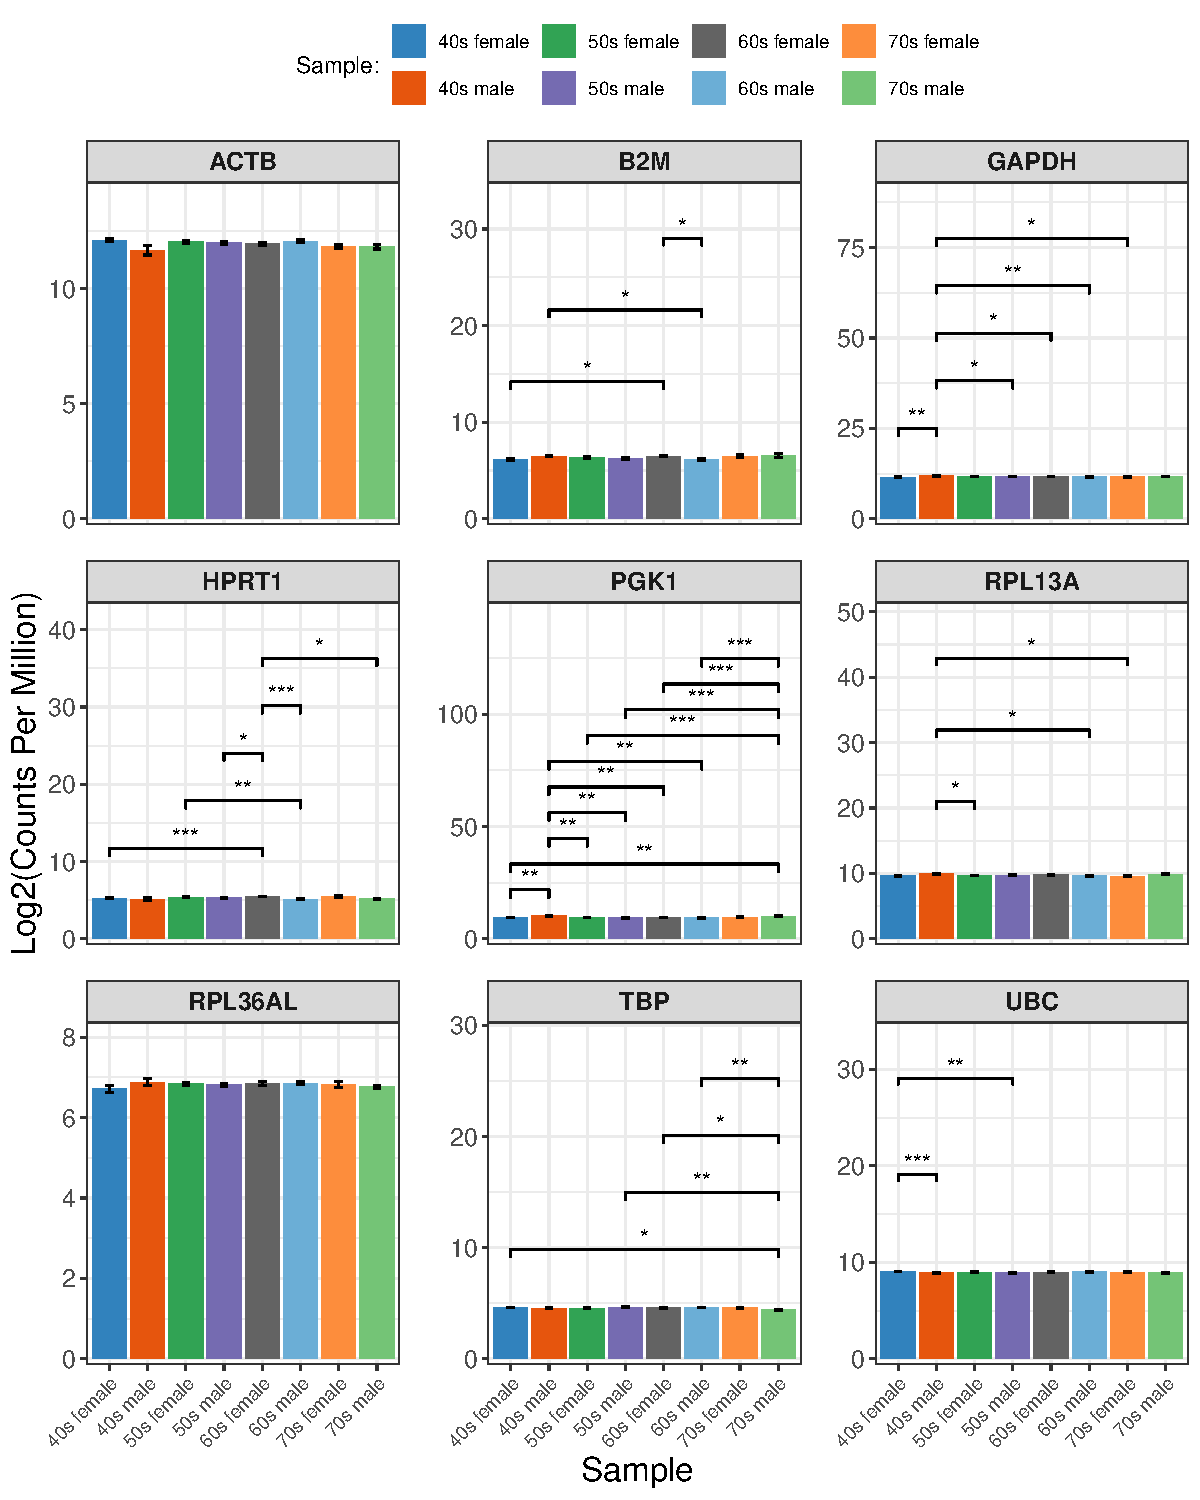
\includegraphics[keepaspectratio]{Final-Project-BIOL806_files/figure-pdf/fig-bargraph-hk-1.pdf}}

}

\caption{\label{fig-bargraph-hk}Expression of Housekeeping Genes}

\end{figure}%

\begin{figure}

\centering{

\pandocbounded{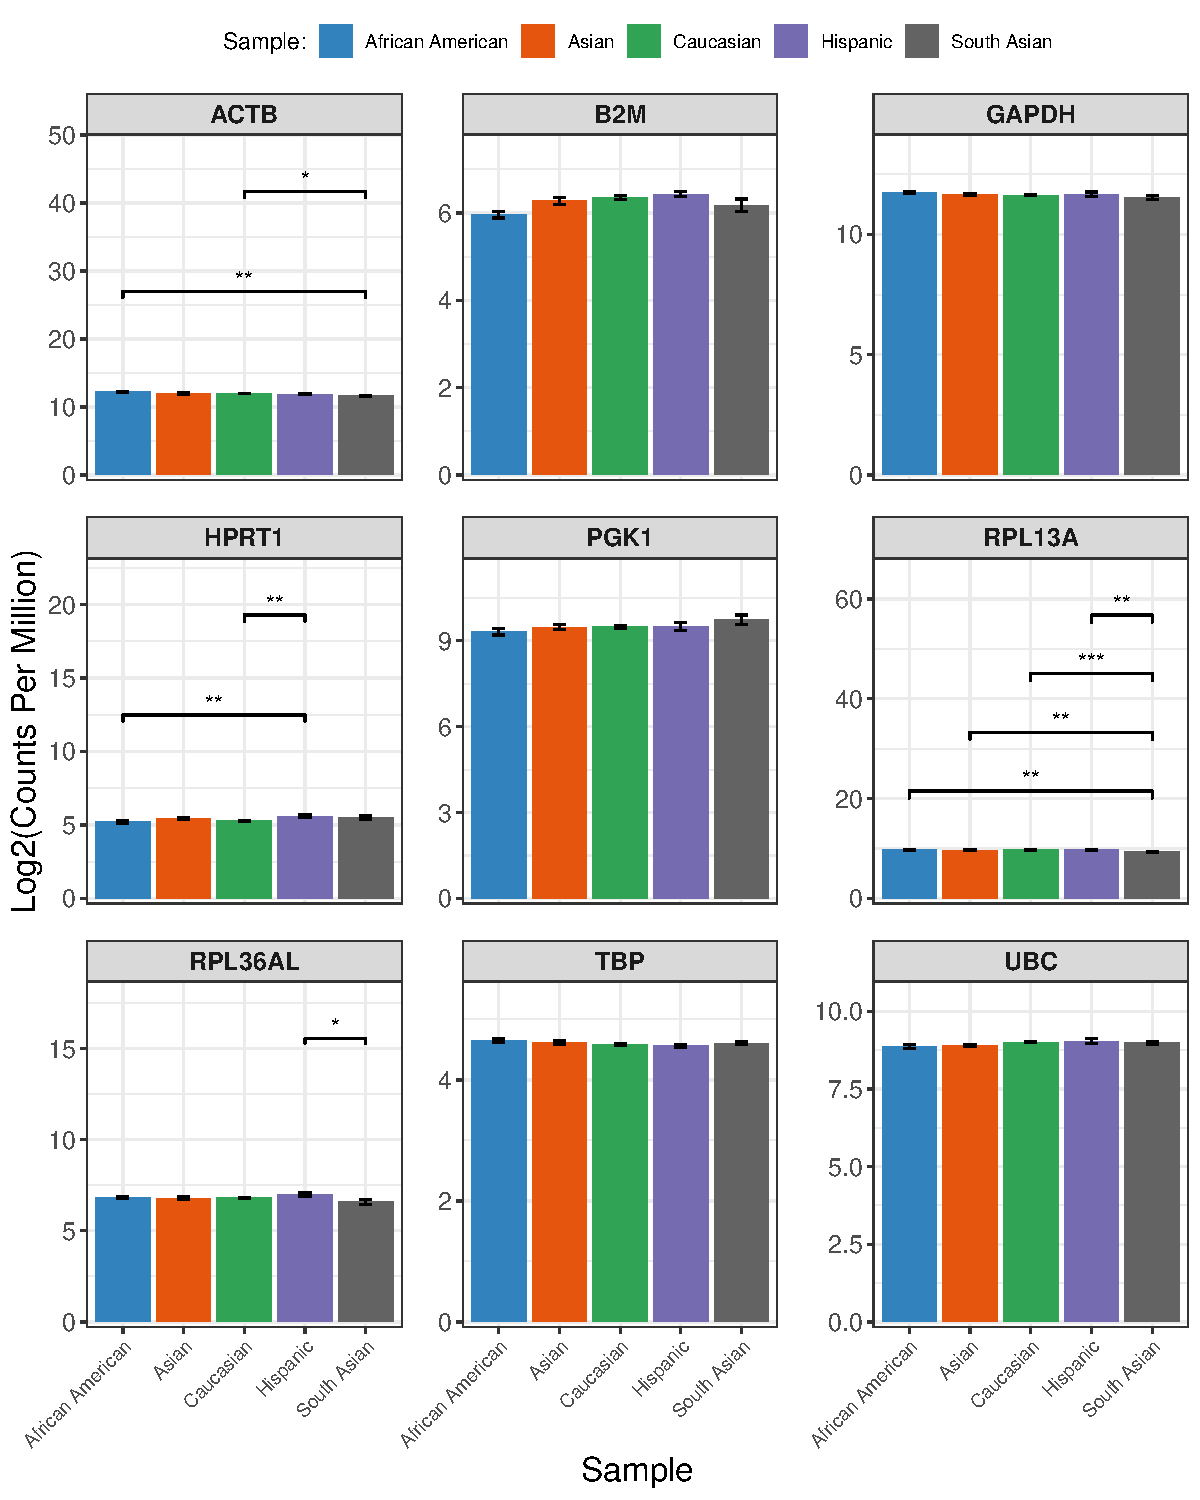
\includegraphics[keepaspectratio]{Final-Project-BIOL806_files/figure-pdf/fig-bargraph-hk-race-1.pdf}}

}

\caption{\label{fig-bargraph-hk-race}Expression of Housekeeping Genes}

\end{figure}%

\begin{verbatim}
# A tibble: 18 x 6
   term    statistic parameter      p.value Gene          p_adj
   <chr>       <dbl>     <dbl>        <dbl> <chr>         <dbl>
 1 age_sex     3.93        7   0.00141      TBP     0.00254    
 2 age_sex     3.93       58.1 0.00141      TBP     0.00254    
 3 age_sex     2.13        7   0.0543       ACTB    0.0611     
 4 age_sex     2.13       57.1 0.0543       ACTB    0.0611     
 5 age_sex     9.93        7   0.0000000478 PGK1    0.000000430
 6 age_sex     9.93       57.2 0.0000000478 PGK1    0.000000430
 7 age_sex     7.26        7   0.00000353   HPRT1   0.0000133  
 8 age_sex     7.26       55.8 0.00000353   HPRT1   0.0000133  
 9 age_sex     4.02        7   0.00117      GAPDH   0.00254    
10 age_sex     4.02       59.0 0.00117      GAPDH   0.00254    
11 age_sex     6.74        7   0.00000443   UBC     0.0000133  
12 age_sex     6.74       68.3 0.00000443   UBC     0.0000133  
13 age_sex     0.806       7   0.586        RPL36AL 0.586      
14 age_sex     0.806      59.5 0.586        RPL36AL 0.586      
15 age_sex     3.61        7   0.00252      B2M     0.00324    
16 age_sex     3.61       62.2 0.00252      B2M     0.00324    
17 age_sex     3.83        7   0.00169      RPL13A  0.00254    
18 age_sex     3.83       59.4 0.00169      RPL13A  0.00254    
\end{verbatim}

\begin{verbatim}
NULL
\end{verbatim}

\section{Discussion}\label{discussion}

\section{Conclusion}\label{conclusion}

\begin{center}\rule{0.5\linewidth}{0.5pt}\end{center}

\section*{References}\label{references}
\addcontentsline{toc}{section}{References}

\phantomsection\label{refs}
\begin{CSLReferences}{1}{0}
\bibitem[\citeproctext]{ref-artyukhov2017}
Artyukhov, A. S., Dashinimaev, E. B., Tsvetkov, V. O., Bolshakov, A. P.,
Konovalova, E. V., Kolbaev, S. N., Vorotelyak, E. A. \& Vasiliev, A. V.
(2017). New genes for accurate normalization of qRT-PCR results in study
of iPS and iPS-derived cells. \emph{Gene}, \emph{626}, 234--240.
\url{https://doi.org/10.1016/j.gene.2017.05.045}

\bibitem[\citeproctext]{ref-carcamo-orive2017}
Carcamo-Orive, I., Hoffman, G. E., Cundiff, P., Beckmann, N. D.,
D'Souza, S. L., Knowles, J. W., Patel, A., Papatsenko, D., Abbasi, F.,
Reaven, G. M., Whalen, S., Lee, P., Shahbazi, M., Henrion, M. Y. R.,
Zhu, K., Wang, S., Roussos, P., Schadt, E. E., Pandey, G., \ldots{}
Lemischka, I. (2017). Analysis of Transcriptional Variability in a Large
Human iPSC Library Reveals Genetic and Non-genetic Determinants of
Heterogeneity. \emph{Cell Stem Cell}, \emph{20}(4), 518--532.e9.
\url{https://doi.org/10.1016/j.stem.2016.11.005}

\bibitem[\citeproctext]{ref-cerneckis2024}
Cerneckis, J., Cai, H. \& Shi, Y. (2024). Induced pluripotent stem cells
(iPSCs): molecular mechanisms of induction and applications.
\emph{Signal Transduction and Targeted Therapy}, \emph{9}(1), 112.
\url{https://doi.org/10.1038/s41392-024-01809-0}

\bibitem[\citeproctext]{ref-panina2020}
Panina, Y., Germond, A. \& Watanabe, T. M. (2020). Analysis of the
stability of 70 housekeeping genes during iPS reprogramming.
\emph{Scientific Reports}, \emph{10}, 21711.
\url{https://doi.org/10.1038/s41598-020-78863-5}

\bibitem[\citeproctext]{ref-poetsch2022}
Poetsch, M. S., Strano, A. \& Guan, K. (2022). Human induced pluripotent
stem cells: From cell origin, genomic stability, and epigenetic memory
to translational medicine. \emph{Stem Cells}, \emph{40}(6), 546--555.
\url{https://doi.org/10.1093/stmcls/sxac020}

\bibitem[\citeproctext]{ref-takahashi2007}
Takahashi, K., Tanabe, K., Ohnuki, M., Narita, M., Ichisaka, T., Tomoda,
K. \& Yamanaka, S. (2007). Induction of pluripotent stem cells from
adult human fibroblasts by defined factors. \emph{Cell}, \emph{131}(5),
861--872. \url{https://doi.org/10.1016/j.cell.2007.11.019}

\bibitem[\citeproctext]{ref-wang2009}
Wang, Z., Gerstein, M. \& Snyder, M. (2009). RNA-seq: A revolutionary
tool for transcriptomics. \emph{Nature Reviews. Genetics}, \emph{10}(1),
57--63. \url{https://doi.org/10.1038/nrg2484}

\bibitem[\citeproctext]{ref-R-tidyverse}
Wickham, H. (2023). \emph{Tidyverse: Easily install and load the
tidyverse}. \url{https://tidyverse.tidyverse.org}

\bibitem[\citeproctext]{ref-R-ggplot2}
Wickham, H., Chang, W., Henry, L., Pedersen, T. L., Takahashi, K.,
Wilke, C., Woo, K., Yutani, H., Dunnington, D. \& van den Brand, T.
(2025). \emph{ggplot2: Create elegant data visualisations using the
grammar of graphics}. \url{https://ggplot2.tidyverse.org}

\bibitem[\citeproctext]{ref-R-dplyr}
Wickham, H., François, R., Henry, L., Müller, K. \& Vaughan, D. (2023).
\emph{Dplyr: A grammar of data manipulation}.
\url{https://dplyr.tidyverse.org}

\bibitem[\citeproctext]{ref-R-scales}
Wickham, H., Pedersen, T. L. \& Seidel, D. (2025). \emph{Scales: Scale
functions for visualization}. \url{https://scales.r-lib.org}

\end{CSLReferences}




\end{document}
